\chapter{Remote entanglement distribution using individual atoms in
cavities}
\label{ch:Borregaard_PRA2015}
%From \cite{Borregaard2015b}
%%%%%%%%%%%%%%%%%%%%%%%%%%%%%%%%%%%%%%%%%%%%%%%%
 

\section{Introduction}

Distribution of entanglement is an essential task in quantum
communication~\cite{kimble,cirac, acin}.  Entanglement can be used to make
highly secure communication channels due to the sensitivity of entangled quantum
systems to external influences~\cite{scarani}. While this sensitivity makes it
possible to detect any attack from an eavesdropper, it also makes it hard to
distribute entanglement over large distances since any noise from the
environment quickly destroys the entanglement. Direct transmission of a quantum signal
suffers from loss and decoherence from the transmission channel, which results
in an exponential decrease of the rate with distance~\cite{briegel}. To overcome
this problem, it has been proposed to use quantum repeaters, where entanglement
is first created over short distances by direct transmission and then stored in
quantum memories until it can be swapped to larger
distances~\cite{briegel,duan3} (See \reffig{fig:figure1}). Much effort has been
devoted to the construction of quantum repeaters based on atomic ensembles,
where the large number of atoms, in principle, enables highly efficient quantum
memories~\cite{sangouard3,cell}. Nonetheless, the limited efficiencies
demonstrated in current experiments with atomic
ensembles~\cite{sangouard3,hammerer} prevents the construction of a practical
quantum repeater based on currently existing setups. 

Single emitter systems such as color centers and trapped ions have also been
considered for quantum repeaters~\cite{childress,sangouard2}. The long coherence
times demonstrated with, e.g. trapped ions make them desirable as quantum
memories. Nonetheless, entanglement needs to be created non-locally between two
memories in the initial step of a repeater. This requires efficient transfer of
information from the quantum memories onto light in the form of single photons.
To this end, it is an advantage to place the emitter inside a cavity, which can
greatly enhance the light-emitter coupling~\cite{acin,ritter}. Entanglement
swapping can then be performed with a cavity mediated CNOT gate
~\cite{pellizari,haroche1} but in this case, the detrimental effect of cavity loss
and spontaneous emission from the emitters may prevent obtaining efficient
entanglement swapping. The parameter characterizing the effect of dissipation in
the emitter-cavity system is the cooperativity, $C$. It has been argued that a
direct implementation of gates in a cavity will make the gate fidelity, $F$,
have a poor scaling of $1-F\sim 1/\sqrt{C}$ \cite{kastoryano,Anders2prl}. To
overcome this problem for current cavities with limited $C$, it has been
suggested to employ entanglement purification after each swap operation to boost
the entanglement but this either requires a large number of resources or a time
consuming sequential generation of purification
pairs~\cite{bennett,deutsch,duan4,pan}.

Here we analyze and compare a number of cavity-based quantum repeaters which
combines various proposals for entanglement generation and cavity-assisted CNOT
gates. We find that the best scheme is where high-fidelity entanglement is
generated using a two-photon detection scheme similar to Ref.~\cite{kimble2} and
swapped to large distances using the heralded CZ-gate proposed in
Ref.~\cite{Borregaard2015a}. The heralded gate enables nearly perfect entanglement
swapping when successful allowing for many swaps without the need of
entanglement purification. As a result, high-rate entanglement distribution is
achieved even for low cooperativities.

Compared to the other cavity-based repeaters, this high-fidelity repeater
achieves up to two orders of magnitude higher secret key rate (see below) for
realistic parameters and large distances ($1000$ km). Specifically, we have
compared to repeaters where entanglement is generated using a single-photon
detection scheme similar to Ref.~\cite{huelga}, which allows for a better rate
at the expense of fidelity. Furthermore, we have considered schemes where
entanglement swapping is achieved using the deterministic CNOT gate suggested in
Ref.~\cite{Anders2prl}, combining it with the local entanglement generation
scheme of Ref.~\cite{Anders1prl}. The advantage of this gate is that the
fidelity scales as $1-F\sim 1/C$, which is a significant improvement from the
$1/\sqrt{C}$ scaling, characterizing the performance of a direct implementation
of gates in a cavity. As a result, long-distance entanglement distribution can
also be achieved with this gate but it requires cooperativities above $100$,
which might be challenging to achieve experimentally. Furthermore, we include
the possibility of initial purification in repeaters based on the single-photon
detection scheme in order to allow for the higher rate of this scheme to
compensate for the lower fidelity compared to the two-photon detection scheme.

To reflect a realistic near-term approach to quantum repeaters, we only consider
scenarios with 2 or 4 qubits per repeater station. For the same reason, we also
do not consider the possibility of intermediate entanglement purification. Here,
initial purification refers to purification in the elementary links (see
\reffig{fig:figure1}) while intermediate purification refers to purification in
the subsequent stages of a repeater. We have numerically optimized all the
considered repeater schemes for a range of cooperativities and distances to find
the highest achievable secret key rate (see below). Note that a similar
optimization of repeater schemes based on dynamical programming was described in
Ref.~\cite{jiang2007}. In that work, both initial and intermediate entanglement
purification was considered assuming high-fidelity operations.  Our optimization
is less detailed since we do not consider intermediate purification. On the
other hand, we include how the errors of the operations depend on the physical
parameters such as the cooperativity and investigate concrete physical
implementations.
Finally, we compare the high-fidelity repeater considered here to both an
ion-trap repeater and one of the best repeaters based on atomic
ensembles~\cite{sangouard3}. For a distance of 1000 km, the high-fidelity
repeater outperforms both of these schemes for $C\gtrsim30$.

\section{High-fidelity quantum repeater}  \label{sec:generation}

We will first describe the details of the high-fidelity quantum repeater, which
we find to have the best performance and later discuss and compare with the
various other schemes. The first step in any quantum repeater is to create
non-local entanglement in the elementary links (see \reffig{fig:figure1}).
\begin{figure} 
\centering
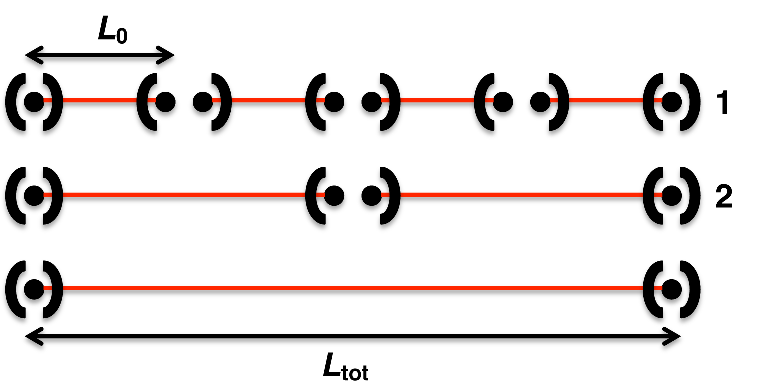
\includegraphics[width=4.0in]{./figs_Borregaard_PRA2015/figure1}
\caption
[The general architecture of a quantum repeater]
{The general architecture of a quantum repeater. The total distance,
over which entanglement should be distributed, is divided into elementary links
of length $L_{0}$ connected by repeater stations pictured as cavities containing
single emitters. After creating entanglement in the elementary links, the
entanglement is swapped to larger distances by combining the elementary links.
The numbers to the right in the figure refers to the swap level of the repeater.
In the first swap level, the four elementary links are connected pairwise to
make two longer links. In the second swap levels these two links are connected
to create entanglement over the total distance. The total number of swap levels
is thus 2 for this depicted setup. }
\label{fig:figure1}
\end{figure} 
To this end, a two-photon detection scheme, as proposed in Ref.~\cite{kimble2},
is considered. The basic setup is shown in \reffig{fig:figure2}(a).
\begin{figure} 
\centering
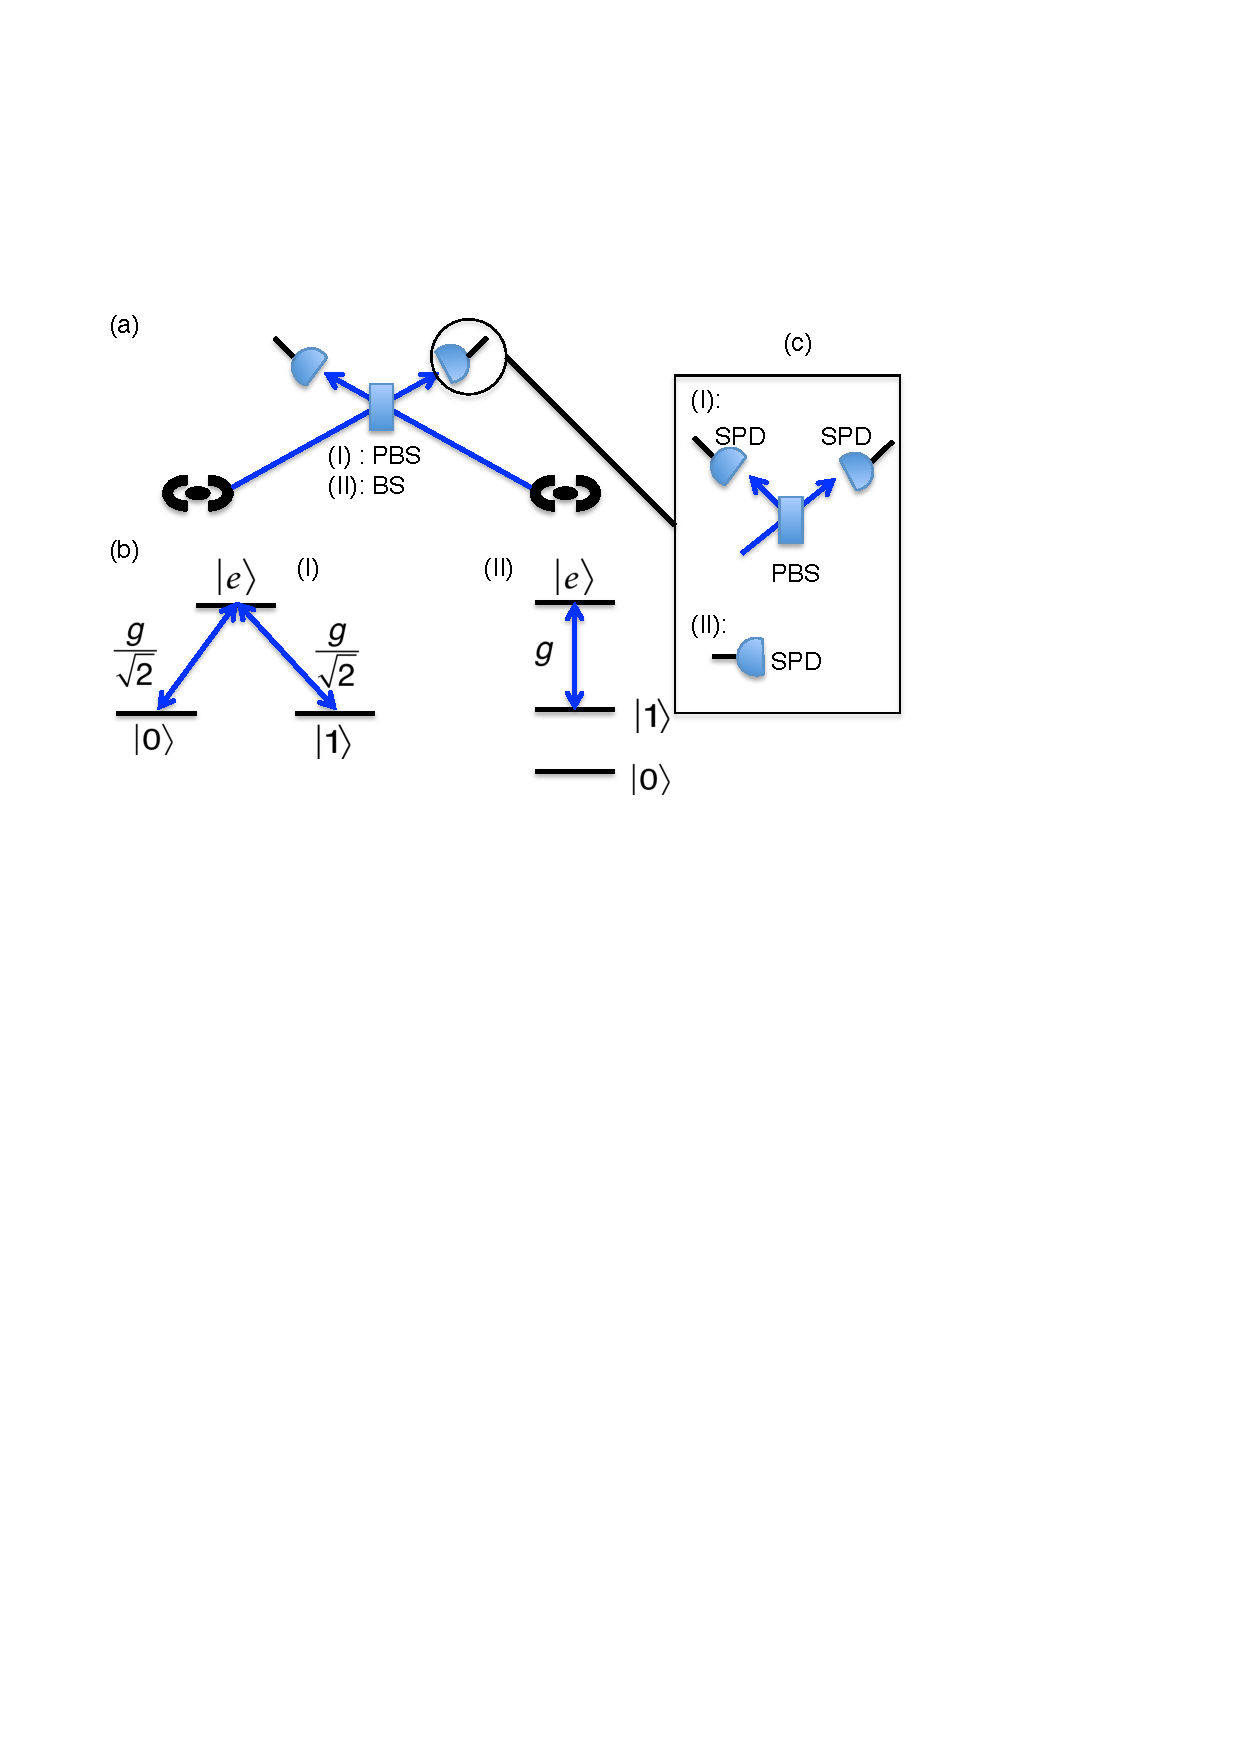
\includegraphics[width=0.7\textwidth]{./figs_Borregaard_PRA2015/figure2}
\caption[Entanglement generation]{Entanglement generation in the elementary
links where emission from two cavities are combined on a beam splitter. (a)
shows the basic setup, (b) shows the level structure of the emitters and (c)
shows the detection setup.  (I) refers to the two-photon detection scheme and
(II) refers to the single-photon detection scheme. Both schemes use a central
station with either (I) three polarizing beam splitters (PBS) and four
single-photon detectors or (II) a single balanced beam splitter (BS) and two
single-photon detectors.  $g$ denotes the cavity coupling. For the two-photon
scheme the levels $\ket{0}$ and $\ket{1}$ are assumed to have equal coupling of
$g/\sqrt{2}$ to the excited state $\ket{e}$.}
\label{fig:figure2}
\end{figure} 
Both emitters are initially prepared in the excited state $\ket{e}$ by a strong
excitation pulse and the cavity is assumed to couple both the
$\ket{e}\to\ket{1}$ and $\ket{e}\to\ket{0}$ transitions with equal coupling
strength $g/\sqrt{2}$ (see \reffig{fig:figure2}(b)). The two transitions are,
however, assumed to produce photons with different polarizations such that the
emission of a cavity photon creates an entangled state between the photon and
the emitter of the form
$\frac{1}{\sqrt{2}}\left(\ket{0}\ket{1_{1}}_{L}+\ket{1}\ket{1_{2}}_{L}\right)$
where $\ket{1_{1}}_{L}$ ($\ket{1_{2}}_{L}$) is the single photon state with
polarization 1 (2). The probability of one of the emitters to emit a photon of
either polarization through the cavity, into an optical fiber transmitting it to
the detection stage during a time interval $[0;T]$ is
\begin{equation} \label{eq:phot1}
P_{\mathrm{phot}}=\frac{4C}{1+4C}\left(1-e^{-\gamma(1+4C)T}\right), 
\end{equation} 
assuming perfect outcoupling to the fiber and that the decay rate of the cavity,
$\kappa$, is much larger than the cavity coupling, $g$. We have here introduced
the cooperativity $C=g^{2}/\kappa\gamma$, where $\gamma$ is the spontaneous
emission rate of the emitters into modes other than the cavity. This is the key
parameter characterizing the performance of the cavity-based repeaters. The
photons are sent from the cavities to a central polarizing beam splitter (PBS).
If two photons of the same polarizations are incident on the PBS, they leave in
different output ports, while photons of different polarization leave in the
same output port. The outputs are then sent to a second set of polarizing beam
splitters and all four outputs of these are finally measured with single photon
detectors (SPD). A click in a detector in each arm heralds the creation of the
Bell state $\ket{\Phi^{+}}=(\ket{00}+\ket{11})/\sqrt{2}$ between the emitters up
to a local qubit rotation. Neglecting dark counts of the detectors, the heralded
fidelity is unity (see App.~\ref{two}) while the success probability of the
scheme is $P_{\mathrm{2click}}=\frac{1}{2}\eta^{2}P_{\mathrm{phot}}^{2}$ with $\eta$
being the total detection efficiency including inefficient outcoupling of the
cavity light, losses in the transmission fibers and imperfect detectors.
Compared to schemes based on single-photon detection (see below) the rate of
this two-photon detection scheme decreases rapidly with decreasing $\eta$. On
the other hand, it has a high fidelity, which is desirable for the subsequent
stages of entanglement swapping, as we will show below.

For entanglement swapping, we find that the best performance is achieved using
the heralded CZ-gate described in Ref.~\cite{Borregaard2015a}. The gate was described
in detail for ${}^{87}$Rb atoms in Ref.~\cite{Borregaard2015a} but it can be easily
generalized to any set of emitters, which have the appropriate level structure
(see \reffig{fig:figure3}). Note that the gate operation relies on only qubit
state $\ket{1}$ coupling to the cavity while the states $\ket{0}$ and $\ket{1}$
had equal cavity couplings in the entanglement generation scheme. To achieve
this change in couplings, the state $\ket{0}$ should be mapped to another level
in between the entanglement generation and the gate operation. For a realization
with alkali atoms where the qubit states would be realized in the hyperfine
grounds states, this could be achieved by applying a magnetic field to resolve
the hyperfine states and applying a microwave pulse resonant with only the
$\ket{0}$ state.
\begin{figure}
\centering
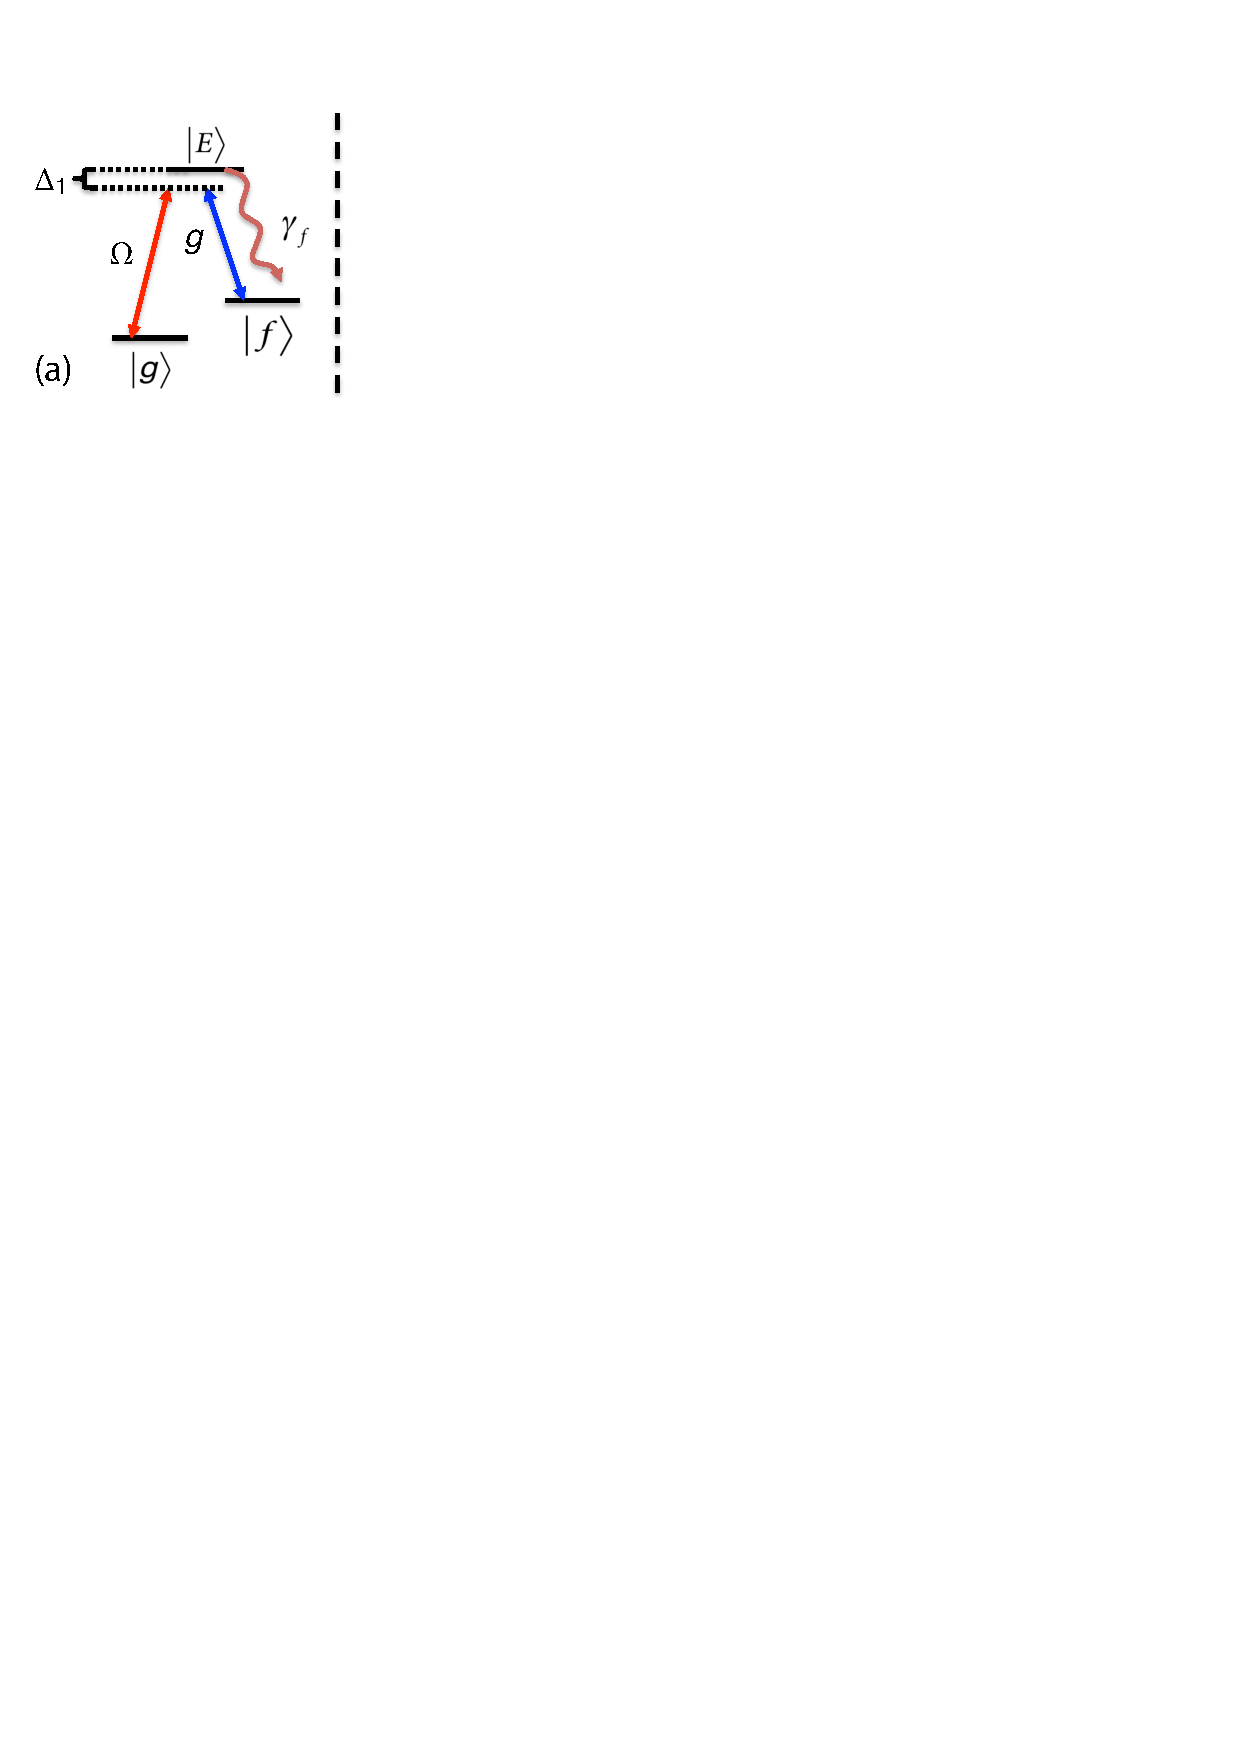
\includegraphics[width=0.3\textwidth]{./figs_Borregaard_PRA2015/figure3a}
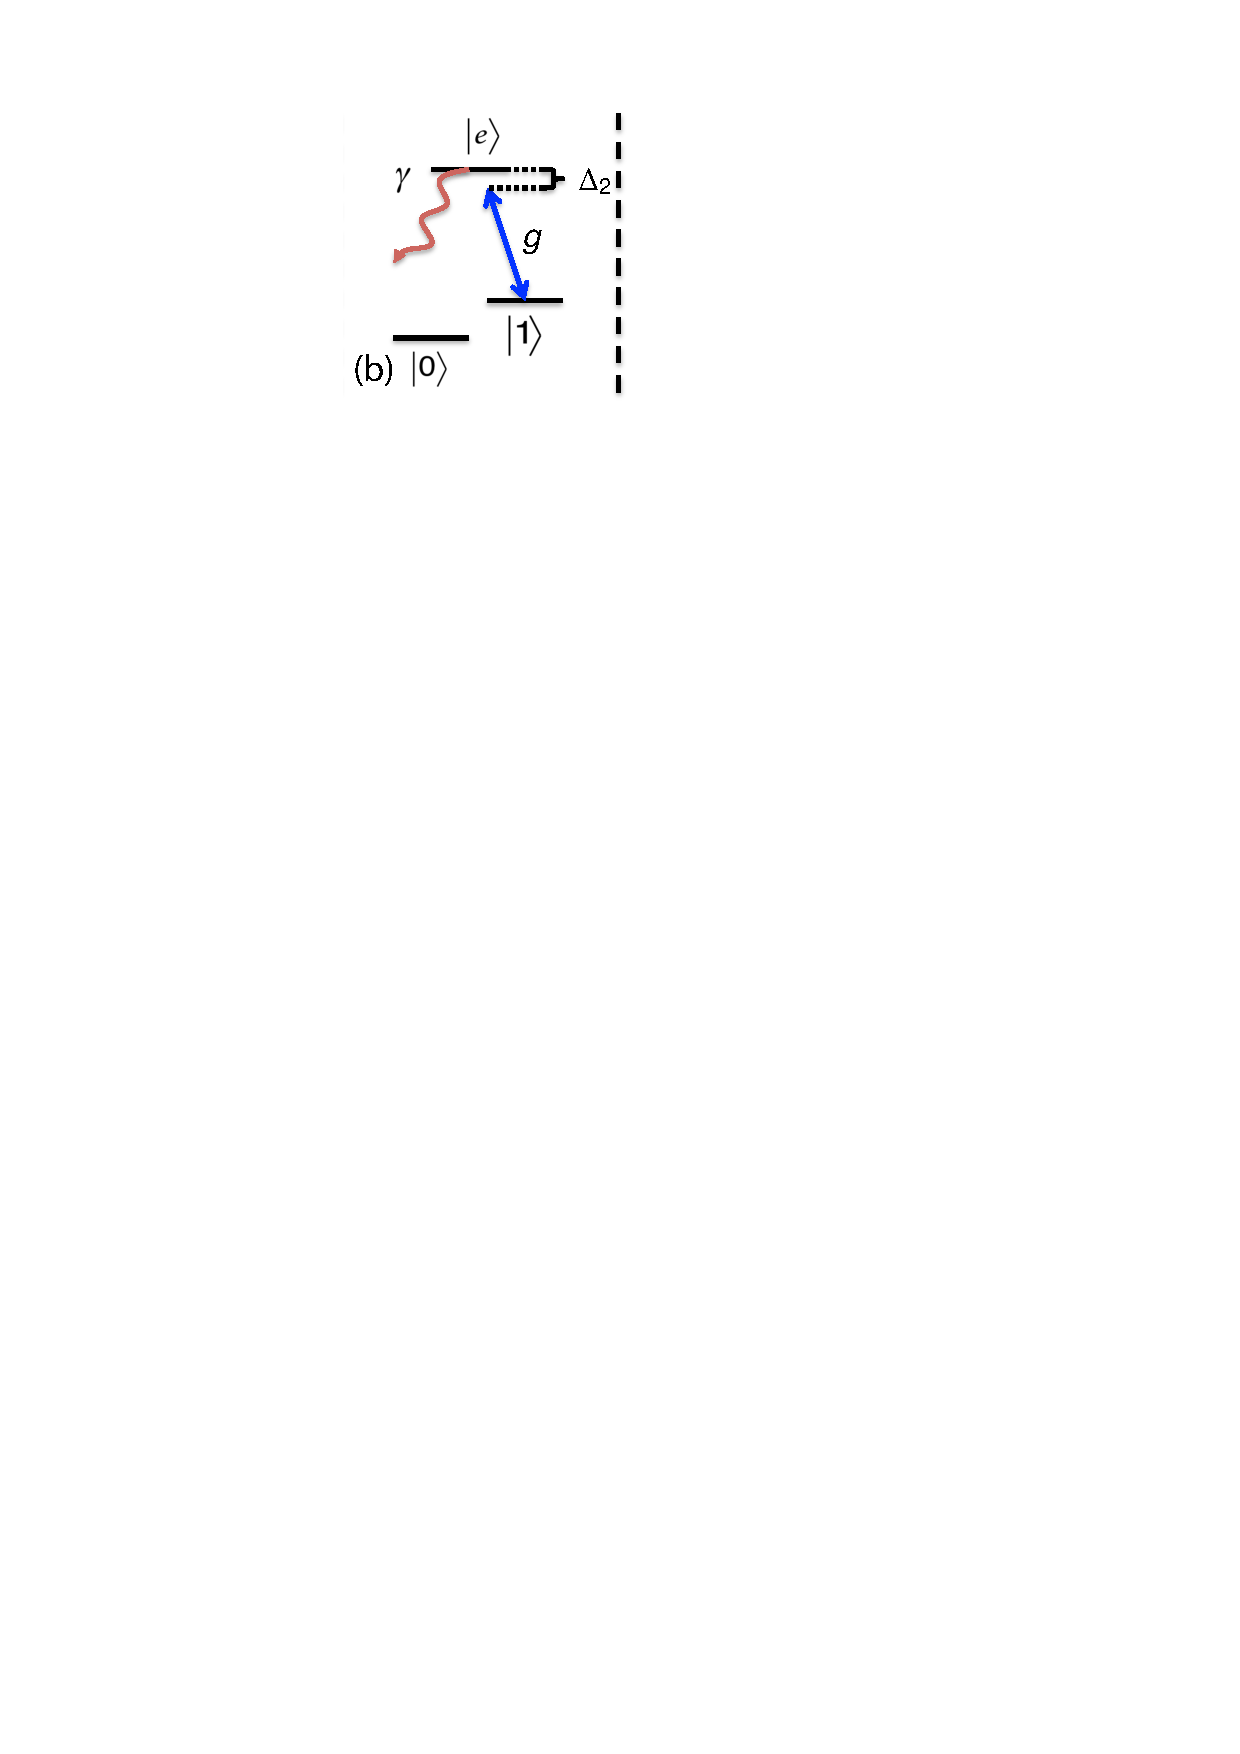
\includegraphics[width=0.3\textwidth]{./figs_Borregaard_PRA2015/figure3b}
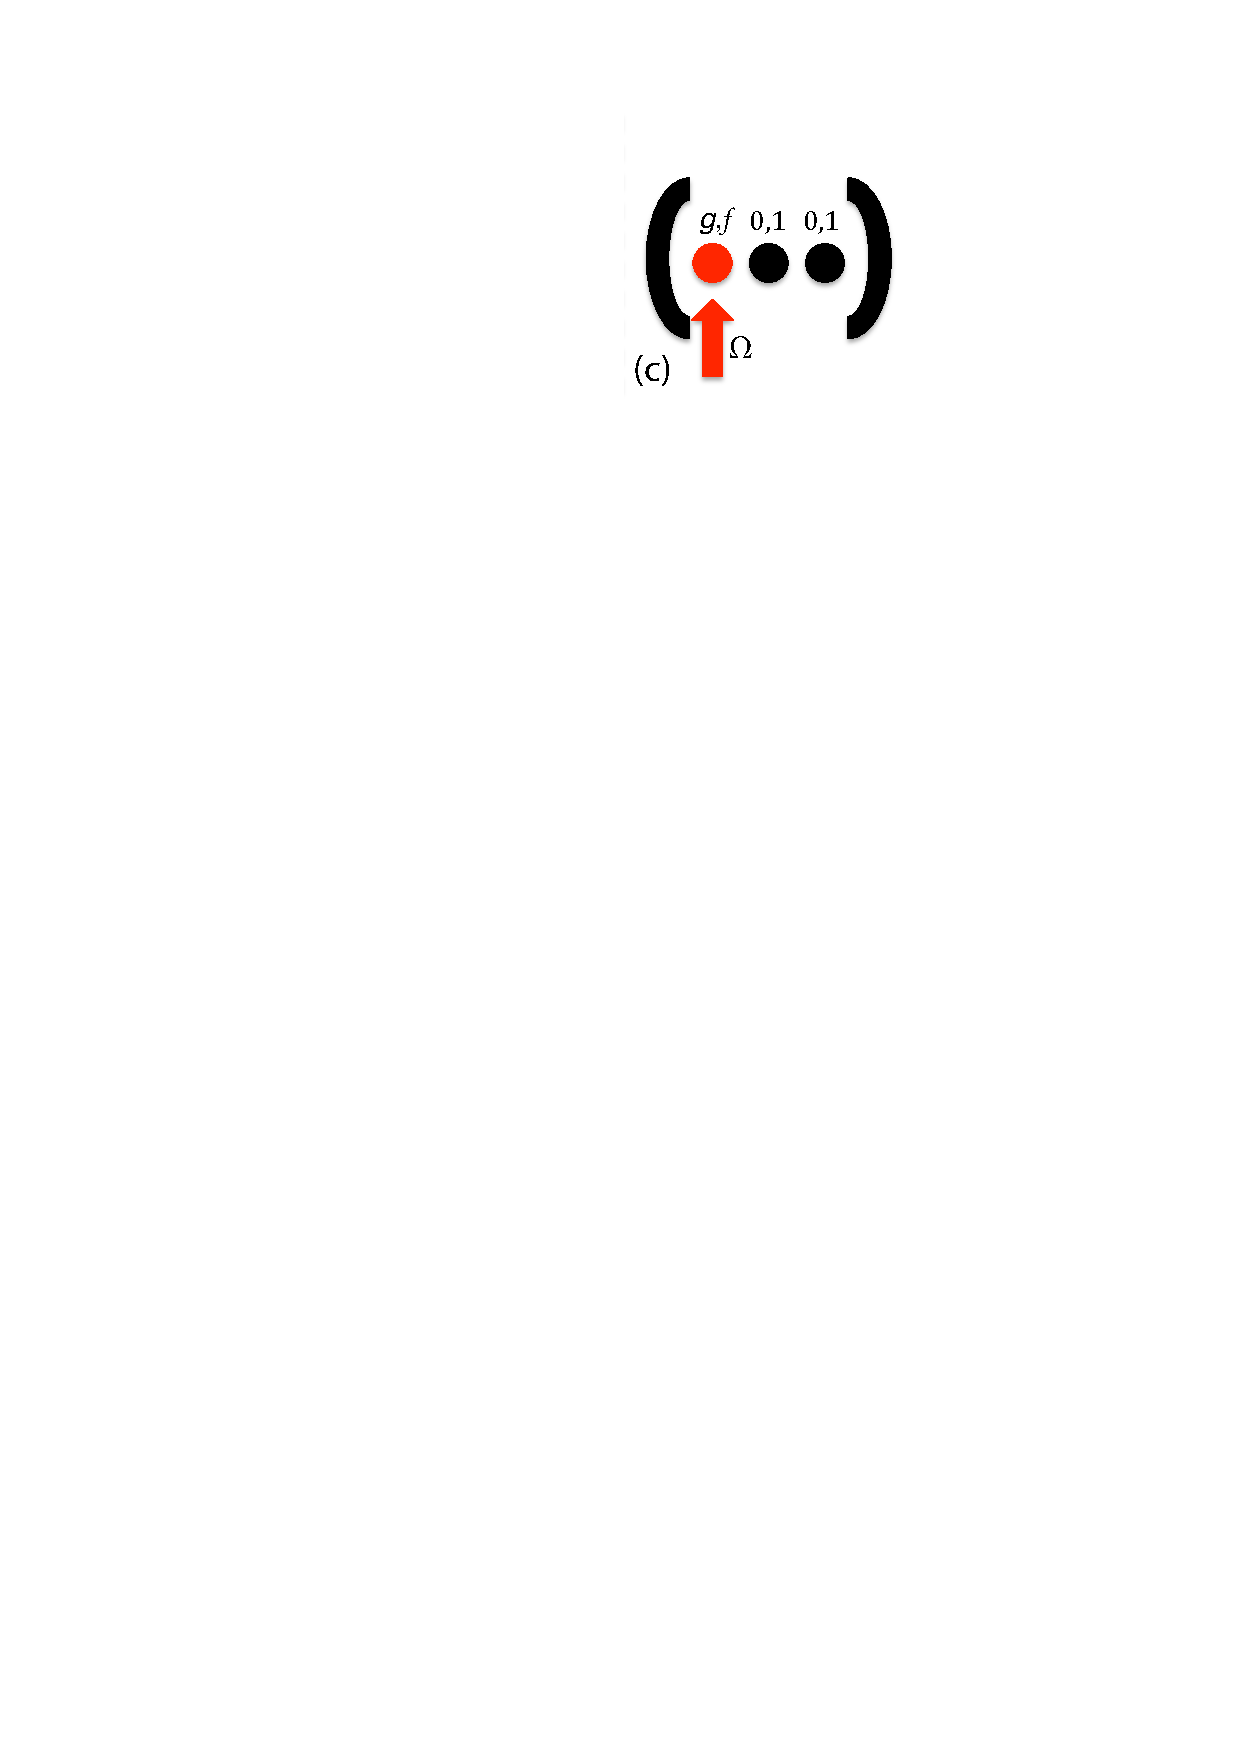
\includegraphics[width=0.3\textwidth]{./figs_Borregaard_PRA2015/figure3c}
\caption
[Schematics of the heralded CZ gate]
{ Schematics of the heralded CZ gate~\cite{Borregaard2015a}. (a) is the level
structure of the auxiliary atom, (b) is the level structure of the qubit atoms
and (c) shows the cavity containing the auxiliary atom and the two qubit atoms.
Assuming that $\ket{E}$ only decays to $\ket{f}$ by e.g. driving the transition
$\ket{g}\to\ket{E}$ with a two photon process, any spontaneous emission or
cavity decay will change the state of the auxiliary atom from the initial state
$\ket{g}$ to $\ket{f}$. The gate is thus conditioned on measuring the auxiliary
atom in state $\ket{g}$ at the end of the gate.}
\label{fig:figure3}
\end{figure}

In the heralded gate, the cavity is assumed to contain two qubit atoms and one
auxiliary atom to facilitate the gate. The auxiliary atom is initialized in a
state $\ket{g}$ that does not couple to the cavity and it would therefore not
interfere with the entanglement generation scheme. By addressing the auxiliary
atom with a weak laser pulse, an AC Stark shift is introduced, which gives a
phase that depends on the state of the qubit atoms. Together with single qubit
rotations, this enables a CZ-gate between the two qubit atoms. Furthermore, the
auxiliary atom can function as an error detector in the sense that any cavity
decay or spontaneous emission changes the state of the atom. Performing a
heralding measurement of the state of the auxiliary atom at the end of the
driving pulse removes all dissipative errors. As a consequence, the gate gets
limited only by non-adiabatic effects. As shown in Ref.~\cite{Borregaard2015a}, a
heralded error below $4\times 10^{-5}$ is possible with a gate time of
$\sim377/(\gamma\sqrt{C})$, where $\gamma$ is the atomic linewidth. The failure
probability of the gate scales as $1/\sqrt{C}$ and the high fidelity thus comes
at the cost of a finite but possibly low failure probability. A CZ gate combined
with single qubit rotations is sufficient to perform direct entanglement
swapping. For simplicity, we assume perfect single qubit rotations and 100\%
efficient measurement of atomic states for all schemes considered. Relaxing this
assumption will in general decrease the rate of all the considered repeater
schemes but schemes with a high number of swap levels, such as the high-fidelity
repeater, will be influenced more on the rate than schemes with a low number of
swap levels.

The advantage of the high-fidelity repeater can be understood by considering the
requirement for reaching a certain threshold fidelity, $F_{\mathrm{final}}$ of the
distributed pair. In this case, the maximum number of swap levels is
$N_\mathrm{max}\sim -\log_{2}(F_{\mathrm{final}}/(\epsilon_{0}+\epsilon_{g}))$,
where $\epsilon_{0},\epsilon_{g}\ll1$ are the errors of the initial entanglement
generation and the entanglement swapping respectively. The combination of the
high-fidelity two-photon detection scheme and the heralded gate thus makes it
possible to have a repeater with many elementary links while maintaining a high
fidelity of the final distributed pair even for low cooperativities since the
error of the heralded gate is still high in this regime.

\subsection{Secret key rate} \label{sec:secret}
We imagine that the distributed entanglement is used to generate a secret key
between two parties referred to as Alice and Bob. There exist various quantum
key distribution schemes \cite{scarani,bennett2,ekert,bruss}, however, the
general idea is that Alice and Bob can exclude that an eavesdropper has any
information about the key by measuring their qubits and comparing results. We
will assume that a six-state version of the BB84 protocol described in Ref.
\cite{bruss} is used to generate the secret key. This protocol consists of three
main steps. First Alice and Bob picks a basis according to some probability
distribution and measure the state of their qubits thereby producing two bit
strings referred to as the \emph{raw key}. Afterwards they compare their choice
of basis and only keep the bits where they chose the same measurement basis
thereby producing a \emph{sifted key}. Finally, Alice and Bob estimate the
information that some eavesdropper could possibly have obtained about their key
and perform privacy amplification \cite{scarani}. If the errors are not too big,
they can obtain a shorter but completely secure key.  For the six-state
protocol, the secret key rate, $r_{\mathrm{secret}}$ can be defined as
\begin{equation}
r_{\mathrm{secret}}=r_{\mathrm{dist}}p_{\mathrm{sift}}f_{\mathrm{secret}},
\end{equation}
where $r_{\mathrm{dist}}$ is the distribution rate of the entangled pairs,
$p_{\mathrm{sift}}$ is the probability that Alice and Bob choose the same
measurement basis and $f_{\mathrm{secret}}$ is the secret key fraction, which
depends on the fidelity of the distributed pairs. We assume a worst case
scenario where the distributed pairs are Werner states of the form
\begin{eqnarray}
\rho&=&F\ket{\Phi^{+}}\bra{\Phi^{+}} +
\frac{1-F}{3}\Big(\ket{\Phi^{-}}\bra{\Phi^{-}}
+\ket{\Psi^{+}}\bra{\Psi^{+}}+\ket{\Psi^{-}}\bra{\Psi^{-}}\Big).
\end{eqnarray}
For such states, it is shown in Ref. \cite{scarani} that the secret key fraction
in the six-state protocol can be estimated in the limit of infinitely long raw
keys to be
\begin{equation} \label{eq:secret2}
f_{\mathrm{secret}}=1-h(\epsilon)-\epsilon+(1-\epsilon)
h\left(\frac{1-3\epsilon/2}{1-\epsilon}\right),
\end{equation} 
where $\epsilon=2(1-F)/3$ and
$h(p)=-p\mathrm{log}_{2}(p)-(1-p)\mathrm{log}_{2}(1-p)$ is the binary entropy.
Eq.~\eqref{eq:secret2} is valid in the limit of perfect sifting and privacy
amplification, which we assume to be the case. Furthermore, we assume an
asymmetric version of the six state protocol, where one basis is used almost all
the time such that $p_{\mathrm{sift}}\approx1$ \cite{scarani}.
\reffig{fig:figure5} shows how the secret key fraction depends on the fidelity
of the distributed pairs.
\begin{figure} 
\centering
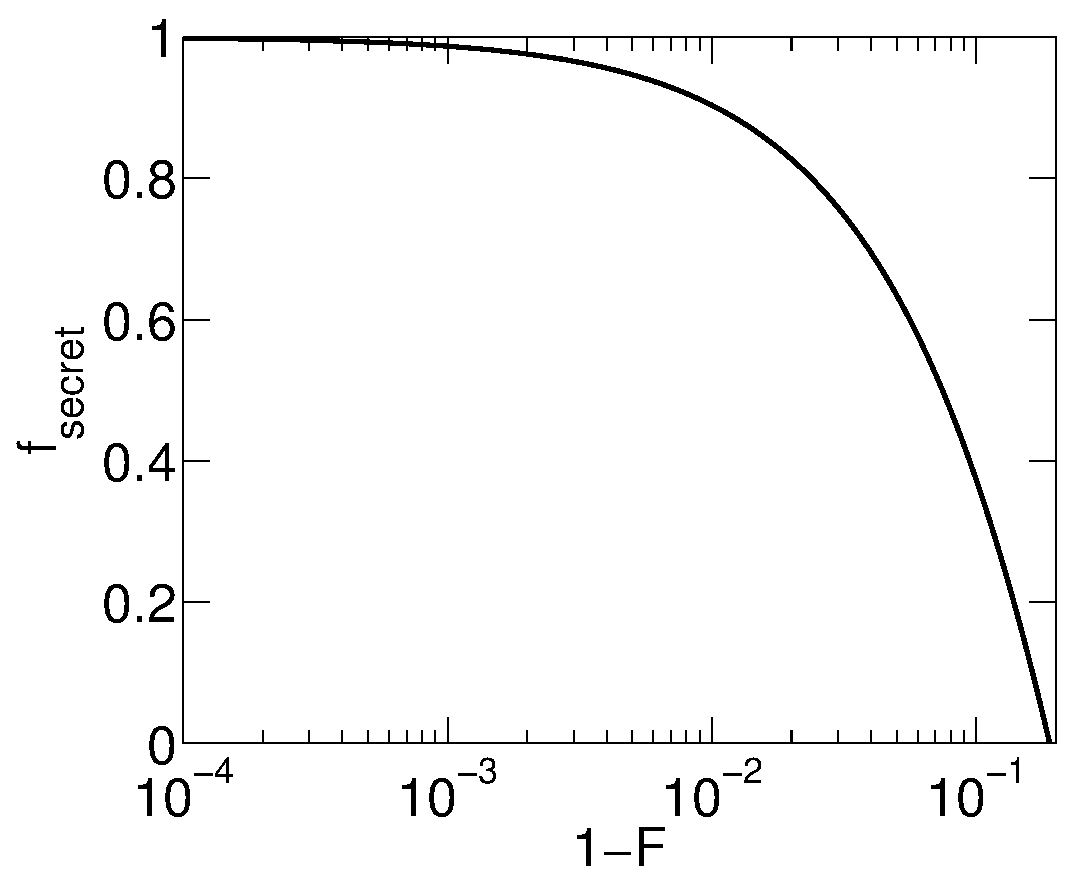
\includegraphics[width=0.6\textwidth]{./figs_Borregaard_PRA2015/figure5}
\caption[Secret key fraction]{Secret key fraction ($f_{\mathrm{secret}}$) as a
function of the infidelity, $1-F$, of the final entangled pair. For
$1-F\gtrsim19 \%$ it is no longer possible to extract a secret key from the raw
keys.}
\label{fig:figure5}
\end{figure} 
As shown in the figure, high-fidelity pairs are required in order to have a
non-vanishing secret key fraction. Again, this points to the high-fidelity
two-photon detection scheme and the nearly error-free heralded entanglement
swapping as the best choice for the repeater.

\subsection{Repeater architecture}

The main goal of the quantum repeater is to overcome the effect of fiber losses.
We model the fiber losses with a transmission efficiency
$\eta_{\mathrm{f}}=e^{-L_{0}/2L_\mathrm{att}}$, where $L_{0}$ is the length of
the elementary links of the repeater and $L_\mathrm{att}$ is the fiber attenuation
length.
$\eta_{\mathrm{f}}$ enters in the total detection efficiency $\eta$ as described
above. For a given resource of $2^{n}+1$ repeater stations, one can either use
all stations in a single repeater with $n$ swap levels or one can construct a
number of parallel, independently operated chains of repeaters with less swap
levels. Increasing the number of swap levels, decreases the fiber losses in the
elementary links and thus increases the rate of entanglement generation. If,
however, the length of the elementary links is already small,  e.g.
imperfect SPD dominates the rate, then increasing the number of swap levels does
not lead to any improvement. In this case it is advantageous to use the extra
repeater stations to make another repeater with less swap levels, which runs in
parallel with the already existing one. To make a proper assessment of the
performance of repeater one should therefore include that adding swap levels
costs resources in the form of additional repeater stations. In our comparison,
we therefore consider a normalized secret key rate,
$\tilde{r}_{secret}=r_{secret}$/(~\#~of stations), which is the secret key rate
divided by the total number of repeater station instead of the bare secret key
rate. To evaluate the performance of the repeater we calculate the achievable
rate $\tilde r_{secret}$ as described in Appendix~\ref{app:rate} with the
assumptions summarized in \tabref{tab:parameter} about fiber losses etc.. The
resulting rate for various swap level used in the repeater is shown in
\reffig{fig:figureX4} as a function of distance. As seen in the figure, the
optimal number of swap level changes with distance while considering the
normalized secret key rate. The rate was calculated as described in
App.~\ref{app:rate} for a cooperativity of 100 with the assumptions summarized
in \tabref{tab:parameter} about fiber losses, detection efficiencies etc. For
distances $\lesssim 150$ km, only a single swap level is needed since the fiber
losses are relatively small while more swap levels are needed as the distance
increases.

\begin{figure} 
\centering
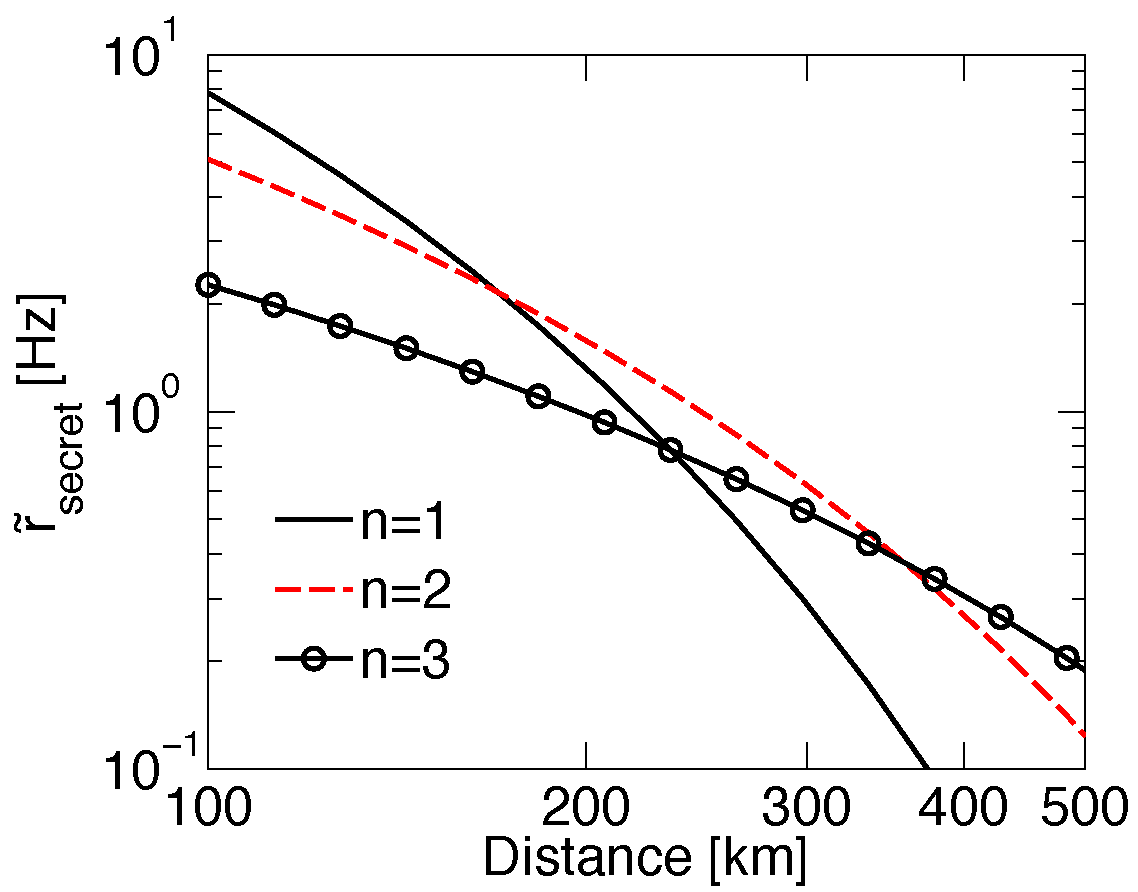
\includegraphics[width=0.65\textwidth]{./figs_Borregaard_PRA2015/figureX4}
\caption[Number of swap levels]{Normalized secret key rate per
station($\tilde{r}_{\mathrm{secret}}$) as a function of the distribution distance
for a high-fidelity repeater consisting of the two-photon entanglement
generation scheme and the heralded gate for entanglement swapping.  We have
considered $n=2,3$ and 4 swap levels and have assumed a cooperativity of $C=$100
and two qubits per repeater station. The secret key rate was calculated as
described in App.~\ref{app:rate} with the assumptions summarized in
\tabref{tab:parameter}.  }
\label{fig:figureX4}
\end{figure} 
  
In most repeater schemes, the qubits in each repeater station are assumed to be
operated simultaneously with half of the qubits being used to generate
entanglement with the neighboring station to each side such that entanglement
attempts in all the elementary links are done simultaneously. We will refer to
this as a \emph{parallel} repeater.  We will, however, also consider another
sequential way of operating the qubits, where all qubits in a station are first
used to make entanglement in one elementary link. After this has been obtained,
all but one qubit are then used to make entanglement over the neighboring link
in the opposite direction. This is referred to as a \emph{sequential} repeater.
The advantage of the sequential repeater is that the rate of the lowest level in
the repeater, the entanglement generation, is increased. This comes at the cost
of a waiting time between entanglement attempts in neighboring links. As the
number of qubits per repeater station increases the sequential repeater will
start to outperform the parallel repeater. We find that this happens with 4
qubits per repeater station (see Sec.~\ref{sec:optim}).

\section{Other cavity based repeaters} \label{sec:other} 

We have found that the high-fidelity repeater that we have described above
outperforms a number of other cavity-based repeater schemes, which can be
constructed with different schemes of entanglement generation and CNOT gates.
Below, we describe the constituents of these other schemes and compare them to
those of the high-fidelity repeater

\subsection{Single-photon entanglement creation} \label{sec:1phot}
It has also been suggested to use single-photon detection schemes similar to
Ref.~\cite{huelga} to generate entanglement in the elementary links. The setup
of a single-photon detection scheme is also shown in \reffig{fig:figure2}. We
assume that the two emitters are initially prepared in a state
\begin{equation}
(1-\epsilon^{2})\ket{00}+\epsilon^{2}
\ket{ee}+\epsilon\sqrt{1-\epsilon^{2}}\left(\ket{0e}+\ket{e0}\right)
\end{equation}    
by a weak excitation pulse such that the excitation probability is
$\epsilon^{2}$. An emitter can then go from state $\ket{e}$ to state $\ket{1}$
by emitting a cavity photon. The emitted photons are collected from the cavities
and combined on a balanced beam splitter (BS) on a central station between the
two cavities. Neglecting losses, the detection of a single photon after the BS
will project the state of the emitters into the Bell state
$\ket{\Psi^{+}}=\frac{1}{\sqrt{2}}\left(\ket{01}+\ket{10}\right)$, up to a
single qubit rotation, in the limit $\epsilon^{2}\ll1$, where we can neglect the
possibility of double excitations. The probability of an emitter to go from
$\ket{e}$ to $\ket{1}$, by emission of a cavity photon during a time interval
$[0;T]$, is $P_{\mathrm{phot}}$ (see Eq.~\eqref{eq:phot1}) under similar
assumptions as in the two-photon scheme described above. Neglecting dark counts
but including losses, the total probability of a single click at the central
station is $P_{\mathrm{1click}}=2\eta
P_{\mathrm{phot}}\epsilon^{2}(1-\epsilon^{2})+(2\eta-\eta^{2})P_{\mathrm{phot}}^{2}\epsilon^{4}$
with $\eta$ being the total detection efficiency as for the two-photon scheme.
The first term is the probability to emit and detect a single photon while the
second term is the probability of emitting two cavity photons but only getting a
single click (we assume that we do not have access to number-resolving
detectors). The probability, to have a single click and have created the state
$\ket{\Psi^{+}}$, is $P_{\mathrm{correct}}=2\eta
P_{\mathrm{phot}}\epsilon^{2}(1-\epsilon^{2})$. The average heralded fidelity
conditioned on a single click is thus
$F_{1}=P_{\mathrm{correct}}/P_{\mathrm{1click}}$. To lowest order in $\epsilon$,
$F_{1}\sim1-(1-\eta/2)P_{\mathrm{phot}}\epsilon^{2}$ while the success probability
is $P_{\mathrm{1click}}\sim2\eta P_{\mathrm{phot}}\epsilon^{2}$. There is thus a
tradeoff set by $\epsilon^{2}$ between the success probability and the fidelity
for the single-photon detection scheme. This is in contrast to the two-photon
detection scheme where $F=1$ regardless of success probability.

The success probability of the single-photon detection scheme is not as
sensitive to the detection efficiency $\eta$ as the two-photon detection scheme
as shown in \reffig{fig:figureX3}.
If the detection efficiency $\eta$ is large, the two-photon scheme is desirable
since it will have both a high success probability and a high fidelity. However,
if $\eta$ is small, the single-photon scheme will be advantageous since it has a
relatively high success probability. Due to the possible high success
probability but limited fidelity of the single-photon scheme, it might be
desirable to combine it with entanglement purification to increase the final
fidelity. In this way, the higher success probability of the single-photon
scheme may compensate the lower fidelity. We have therefore considered the possibility
of initial entanglement purification in repeaters based on the single-photon
detection scheme as described below.

\subsection{Initial purification}
Based on a detailed analysis of the various errors that limit the fidelity for
the single-photon scheme including dark counts of the detectors (see
App.~\ref{single} for details), we find that the purification protocol of
Ref.~\cite{bennett} effectively corrects for the errors in the single-photon
scheme and we assume that this is used for the initial purification. However, as
pointed out in Ref.~\cite{nickerson} an improved fidelity, at the expense of a
factor of $\sim2$ in the success probability, can be obtained by only accepting
outcomes where the two heralding qubits are found in state $\ket{1}\ket{1}$
instead of also accepting $\ket{0}\ket{0}$ outcomes. We will also consider this
modification to the purification protocol of Ref.~\cite{bennett}. The protocol
relies on a CNOT operation, which we assume to be made with the same gate used
to perform the subsequent entanglement swapping (see below). To reflect the most
realistic near-term quantum repeaters we consider at most 4 qubits per repeater
stations. We therefore assume that the purification is performed in a pumping
scheme~\cite{briegel2}, where the fidelity of a single pair is pumped by
combining it with pairs of lower fidelity since this requires the lowest number
of qubits per station.

The effect of combining the single-photon scheme with initial purification is
shown in \reffig{fig:figureX3} where, for simplicity, the purification is
assumed to be performed with a deterministic gate with perfect fidelity and
without the modification of Ref.~\cite{nickerson}. If high fidelity pairs are
desired for, e.g., a repeater with many swap levels, entanglement purification
can increase the rate of the entanglement generation. For high collection
efficiencies it is, however, desirable to use the two photon scheme since this
has a higher rate. In particular, the two photon scheme becomes desirable if
high fidelity pairs are required.

\begin{figure} 
\centering
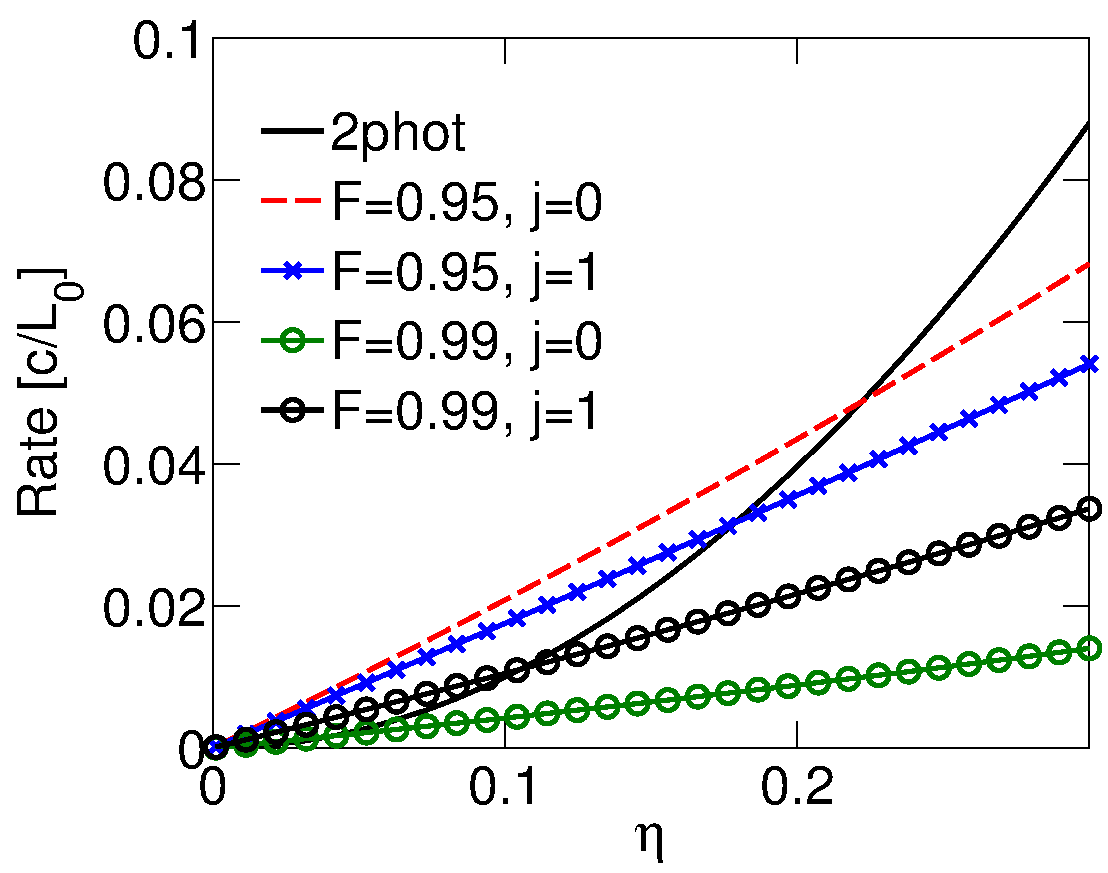
\includegraphics[width=0.6\textwidth]{./figs_Borregaard_PRA2015/figureX3}
\caption[Purification]{Rate of entanglement generation for the two-photon scheme
and the single-photon scheme with target fidelity $F\geq0.95$ and $F\geq0.99$
both without purification ($j=0$) and with one round of purification ($j=1$).
The rate is shown as a function of the total detection efficiency $\eta$. We
have neglected dark counts and assumed that the CNOT gate is deterministic and
have perfect fidelity. The rate has been calculated as described in
App.~\ref{app:rate}. Furthermore, we have assumed that each repeater station
contains 4 qubits, which are either used for purification or to increase the
rate of the entanglement generation. }
\label{fig:figureX3}
\end{figure} 

\subsection{CNOT gates} \label{sec:CNOTgate}

In our analysis, both the initial purification and the subsequent entanglement
swapping involves a cavity-based CNOT gate. Besides the heralded CNOT gate used
in the high-fidelity repeater, which we will refer to as \emph{gate 1}, a
deterministic cavity-based gate proposed in Ref.~\cite{Anders2prl} could be
used. Combining the gate scheme of Ref.~\cite{Anders2prl} with the local
entanglement generation scheme of Ref.~\cite{Anders1prl} results in a
deterministic CNOT gate with an error scaling as $1/C$.  We will refer to this
gate as \emph{gate 2}. This gate does not require an auxiliary atom as gate 1
but rather two auxiliary levels in the qubit atoms as shown in
\reffig{fig:figure4}(a).
\begin{figure}
\centering
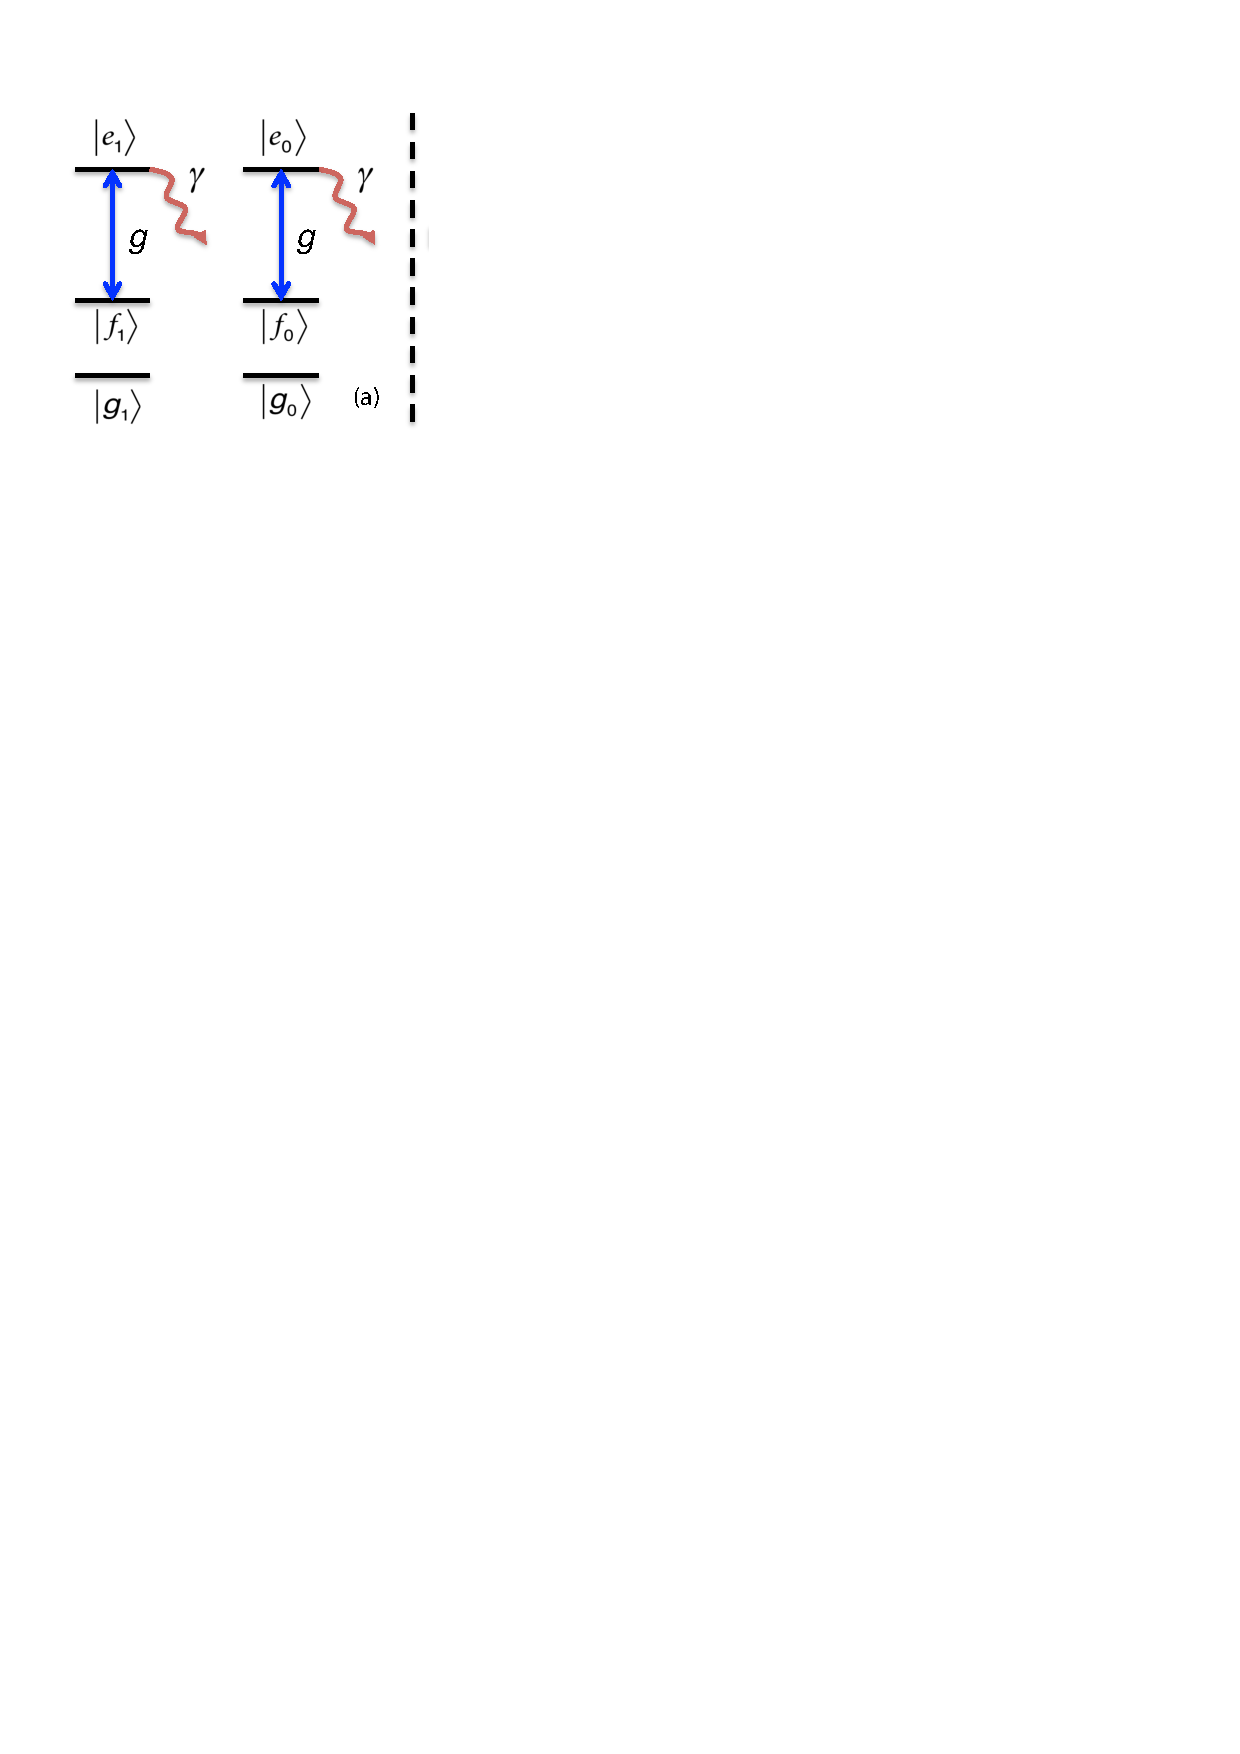
\includegraphics[width=0.4\textwidth]{./figs_Borregaard_PRA2015/figure4a}
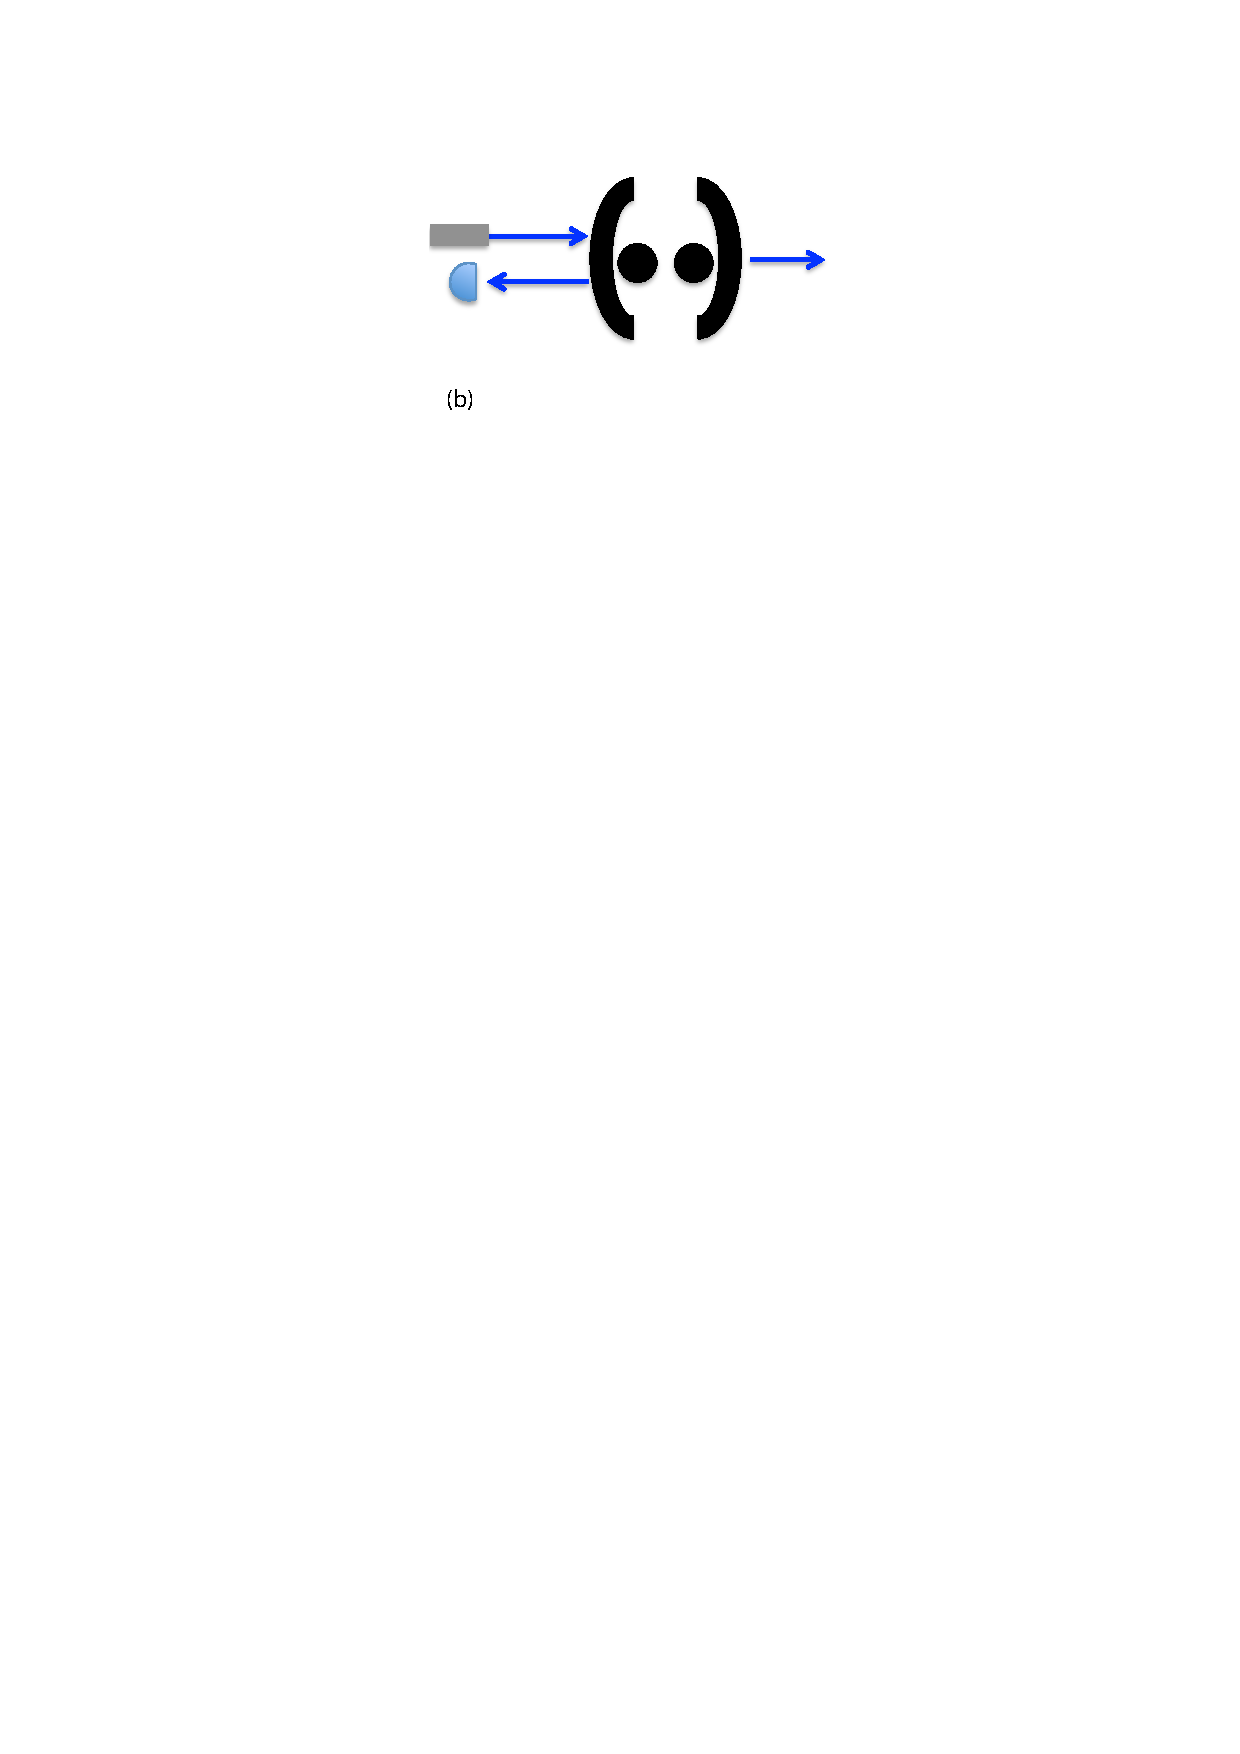
\includegraphics[width=0.4\textwidth]{./figs_Borregaard_PRA2015/figure4b}
\caption[CNOT gate structure]
{Deterministic gate based on reflection and
teleportation based CNOT operation~\cite{Anders1prl,Anders2prl}(a) Level
structure of the qubit atoms. The levels $\ket{r_{0}}$ and $\ket{r_{1}}$ where
$r=g,f$ or $e$ are assumed to be degenerate such that the quantum information is
encoded in the horizontal degrees of freedom. (b) The setup to create
entanglement between the level states $\ket{g},\ket{f}$ of the atoms. Weak
coherent light is sent onto the cavity and any reflected light is measured with
a SPD. }
\label{fig:figure4}
\end{figure}
In this scheme, the quantum information is stored in the horizontal/qubit degree
of freedom (subscripts $0$ and $1$) and the vertical/level degree of freedom
(denoted $g$ and $f$) is used to make an entanglement assisted CNOT gate between
the atoms. Separating the qubit degree of freedom from the level degree of
freedom, the gate works by ideally making the transformation
\begin{equation} \label{eq:transgate1}
\ket{q1}\ket{q2}\otimes\ket{gg}\to
\ket{q1}\ket{q2}\otimes\frac{1}{\sqrt{2}}\left(\ket{gf}+\ket{fg}\right),
\end{equation} 
where $\ket{g},\ket{f}$ denote the vertical states and $\ket{q1}$ ($\ket{q2}$)
is the qubit state of the first (second) qubit, which could be entangled with
atoms at neighboring repeater stations. The entanglement between the levels
$\ket{g}$ and $\ket{f}$ can be used to make a CNOT gate, if the levels of the
atoms can be measured non-destructively, i.e. without revealing any information
about the qubit state as described in Ref.~\cite{Anders2prl}. Both the
transformation shown in Eq.~\eqref{eq:transgate1} and the non-destructive
measurements can be obtained by sending a weak coherent pulse onto a two-sided
cavity and detecting any reflected light (see \reffig{fig:figure4}(b) and
App.~\ref{app:cnot}). If the light is resonant with the empty cavity mode, atoms
in $\ket{f}$ will shift the cavity resonance. Consequently, photons will be
reflected and constitutes a QND measurement of the presence of atoms in
$\ket{f}$. Spontaneous emission from the atoms will limit the fidelity of the
gate to $F\sim1-1.2/(\eta_{\mathrm{d}}C)$, where $\eta_{\mathrm{d}}$ is the
detection efficiency and $C=g^{2}/\kappa\gamma$ is the cooperativity. The gate
time is limited by the time of the single qubit rotations and the coherent
pulses.  We assume that this gives a gate time on the order of 10 $\mu$s.

As a benchmark, we also consider a naive approach where a direct gate between
two qubits is made in a cavity without the use of an auxiliary atom or auxiliary
atomic states. To characterize such a gate, we consider a situation where the
setup of gate 1 is used to make a deterministic gate by simply ignoring the
heralding condition. We will refer to this gate as \emph{gate 3}. For such a
gate, we find that the gate fidelity will scale as $1-F\sim3/\sqrt{C}$ and the
time of the gate will be limited by the time of the single qubit rotations which
we assume to be $\sim10$ $\mu$s.

The characteristics of the three gates we consider are summarized in
\tabref{tab:table2} and illustrated in \reffig{fig:figureX2}.
\begin{table} 
\centering
\begin{tabular}{|c|c|c|c|}
\hline
Gate & Fidelity & Probability & Gate time  \\ \hline
1  & $F=4\cdot10^{-5}$ & $P_{g}\sim1-6/\sqrt{C}$ & $377/(\gamma\sqrt{C})$+10 $\mu$s\\ \hline
2 & $F\sim1-1.2/(\eta_{\mathrm{d}}C)$ & $P_{g}=1$ &10 $\mu$s  \\ \hline
3 & $F\sim1-3.6/\sqrt{C}$ & $P_{g}=1$ &10 $\mu$s \\ \hline
\end{tabular}
\caption
[Characteristics of the three gates]
{Characteristics of the three gates considered for the
cavity-based repeaters. $C$ is the cooperativity of the atom-cavity system and
$\eta_{\mathrm{d}}$ is the single photon detection efficiency in gate 2. The time
of the single qubit rotations is assumed to be 10 $\mu$s. }
\label{tab:table2}
\end{table}
\begin{figure} 
\centering
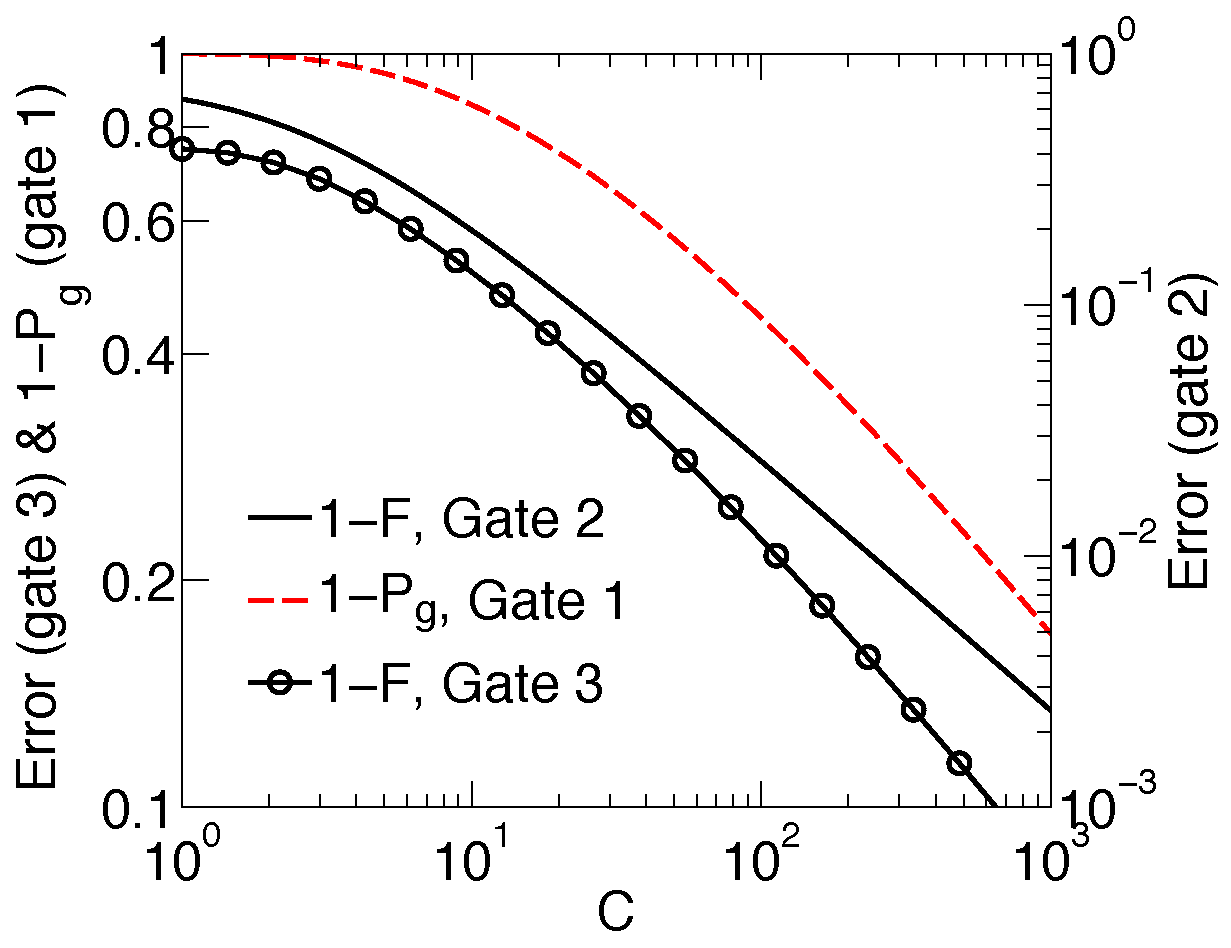
\includegraphics[width=0.6\textwidth]{./figs_Borregaard_PRA2015/figureX2}
\caption[CNOT gates comparison]{Characteristics of the three gates described in
the text. The errors of gate 2 (black/solid line, right axis) and gate 3
(black/circled line, left axis) are shown as a function of the cooperativity.
The error is defined as $1-F$ where $F$ is the fidelity of the gate. We have
assumed $\eta_{d}=0.5$ for the error of gate 2. Gate 1 has conditional fidelity
$\sim1$ but a finite failure probability $1-P_{g}$ which is also shown as a
function of cooperativity (red/dashed line, left axis).}
\label{fig:figureX2}
\end{figure} 
It is clear, that a repeater based on gate 3 will never be advantageous but we
consider it as a reference since the physical requirements for implementing this
gate are less than for gate 1 and 2, which requires either an auxiliary atom or
auxiliary atomic levels.

\section{Numerical optimization} \label{sec:optim}
We have numerical optimized the secret key rate per repeater station for both
the high-fidelity repeater and all other cavity-based repeaters consisting of
the elements considered in Sec.~\ref{sec:other}. The secret key rate is
calculated as described in Sec.~\ref{sec:secret} and App.~\ref{app:rate}. It
depends on experimental parameters such as the efficiency of single photon
detectors, dark count rates. The values of these parameters are assumed
fixed and are thus not part of the optimization.  All the experimental
parameters are summarized in \tabref{tab:parameter} together with the values
assumed in the optimizations. We have assumed fiber transmission losses for
telecom wavelengths, which may require wavelength conversion techniques
\cite{boris}.
{
\ssp
\begin{table}
\centering
\begin{tabular}{| c | c| p{8cm} | }
\hline
Parameter & Value & Description \\ \hline
$\gamma$ & $2\pi \cdot 6$ MHz & Spontaneous emission rate of atoms. This enters in the probability of emitting a photon in the entanglement generation schemes (see Eq.~\eqref{eq:phot1}) and in the gate time of gate 1 and 2. \\ \hline
$\eta_{\mathrm{d}}$ & $50\%$ & Combined efficiency of SPD detectors and outcoupling of light from the cavities. This enters in the total detection efficiency $\eta$ in the entanglement generation schemes since $\eta=\eta_{\mathrm{d}}\eta_{\mathrm{f}}$. It also enters the fidelity of gate 2. \\ \hline 
$L_{att}$ & 22 km  & Attenuation length of the fibers. The total transmission probability over a length $L$ is assumed to be $\eta_{\mathrm{f}}=e^{-L/L_{att}}$. The value assumed corresponds to telecom wavelengths.  \\ \hline
$\tau_{\mathrm{local}}$ & 10 $\mu$s & Time of local qubit operations  \\ \hline
$r_{dark}$ & 25 Hz & Dark count rate of SPD detectors. We include dark counts in the entanglement generation step but not in the gate operations since the gate operations are assumed to be fast.  \\ \hline
$c$ & $2\cdot 10^{5}$ km/s & Reduced speed of light in the transmission fibers \cite{sangouard3}. \\ \hline
\end{tabular}
\caption[Parameters in the numerical optimization]{Experimental parameters which
influence the rate and fidelity of the repeaters. The second column gives the
values used in all optimizations.}
\label{tab:parameter}
\end{table}
}
The free parameters in the optimizations are the number of swap levels, the
number of purifications with/without the modification of Ref.~\cite{nickerson}
and whether a parallel or sequential repeater protocol is used. In the
optimizations, we calculate the secret key rate on a grid of all these
parameters and pick the combination giving the highest rate.
\reffig{fig:figureX6} shows a specific example where the combination of the
single-photon scheme with gate 2 is investigated for a parallel repeater and a
cooperativity of 100.
\begin{figure} 
\centering
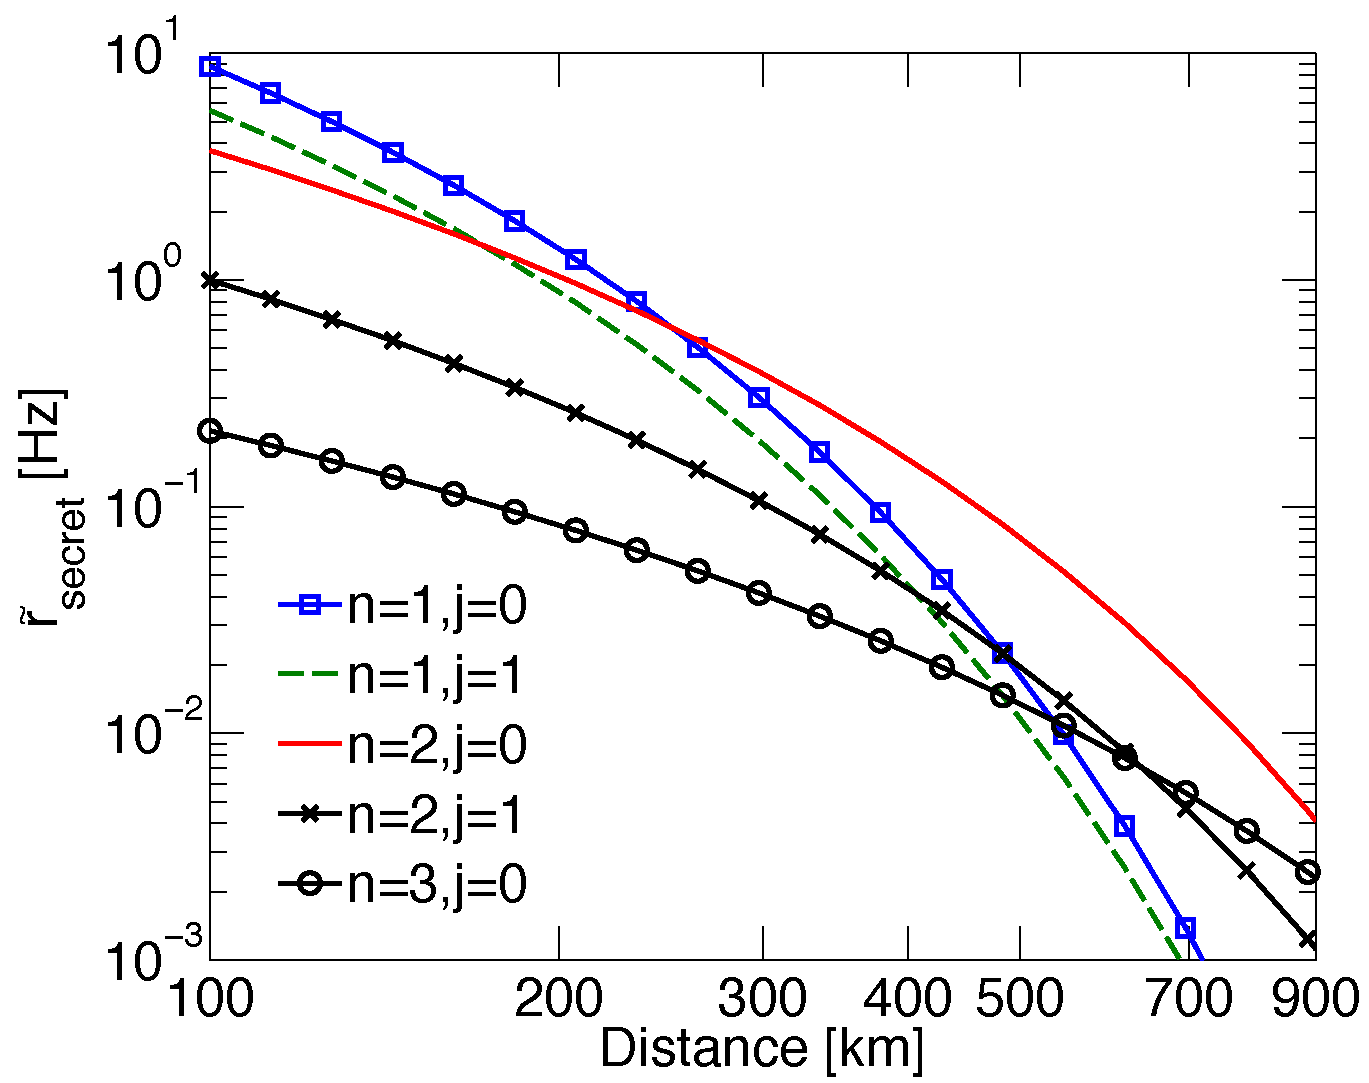
\includegraphics[width=0.65\textwidth]{./figs_Borregaard_PRA2015/figureX6}
\caption[Example of repeater architecture]{Normalized secret key rate per
station($\tilde{r}_{\mathrm{secret}}$) as a function of the distribution distance
(Distance) for a parallel repeater based on the single photon generation scheme
and gate 2. The cooperativity was assumed to be 100 and we assumed 4 qubits per
repeater station. The optimal number of swap levels ($n$) and purification
rounds ($j$) for a given distance can be directly read off from the plot as the
combination giving the highest rate. Note that because the gate fidelity is
limited, curves with $j=2$ and $n=3,j=1$ are not shown since they result in a
much lower secret key rate. The purification schemes was considered to be
without the modification of Ref.~\cite{nickerson}.}
\label{fig:figureX6}
\end{figure} 
The number of swap levels and purifications, giving the highest rate for a
specific distance, can be directly read off from the figure. The same
calculations are then done for a sequential repeater protocol and compared to
the parallel repeater protocol with/without the modified purification in order
to find the highest rate for this specific combination of entanglement
generation scheme and CNOT gate. This is done for all combinations of
entanglement generation schemes and CNOT gates. The optimal evolution time, $T$,
and excitation probability, $\epsilon$, in the entanglement generation schemes
are found for each grid point using a built-in numerical optimization in the
program MATLAB.
The key parameter, determining the performance of the CNOT gates, is the
cooperativity (see \tabref{tab:table2}). We therefore optimize for
cooperativities $C\in[10;1000]$ and distances between 100 km and 1000 km.
Finally, the optimizations are performed for both 2 qubits per repeater station
and 4 qubits per repeater station. Note that the auxiliary atom used in gate 1
is not counted as a qubit and schemes based on this gate thus in principle
contain an additional atom per repeater station.

We model the effect of the non-perfect gates, as depolarizing channels such that
the output of a gate operation described by a unitary $U_{\mathcal{S}}$ working
on a set $\mathcal{S}$ of two qubits is
\begin{equation} \label{eq:gateerror}
\tilde{\rho}=F'U_{\mathcal{S}}\rho
U^{\dagger}_{\mathcal{S}}+\frac{1-F'}{4}\left(\mathrm{Tr}
\left\{\rho\right\}_{\mathcal{S}}\otimes\mathds{1}_{S}\right),
\end{equation}
where $F=F'+(1-F')/4$ is the fidelity of the gate, $\mathds{1}_{\mathcal{S}}$ is
the identity matrix of the set, $\mathrm{Tr}\{\ldots\}_{\mathcal{S}}$ is the
trace over the set and $\rho$ is the initial density matrix describing the system
before the gate operation. We use Eq.~\eqref{eq:gateerror} to propagate the
density matrix from the entanglement generation (see
App.~\ref{single}-\ref{two}) through the steps of initial purification and
entanglement swapping and calculate the average fidelity of the distributed
pairs. To calculate the secret key fraction, we treat the distributed pairs as
Werner states as described in section \ref{sec:secret}.
\begin{figure} [H]
\centering
% 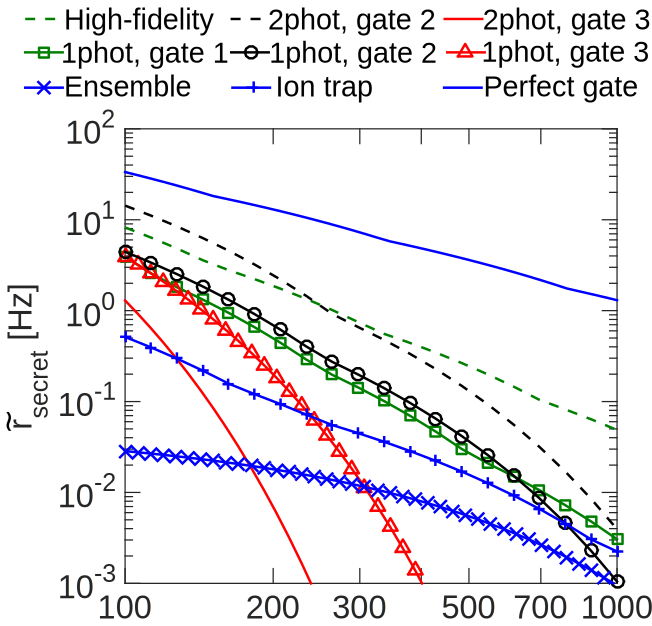
\includegraphics[width=0.48\textwidth]{./figs_Borregaard_PRA2015/figureX7a}
% 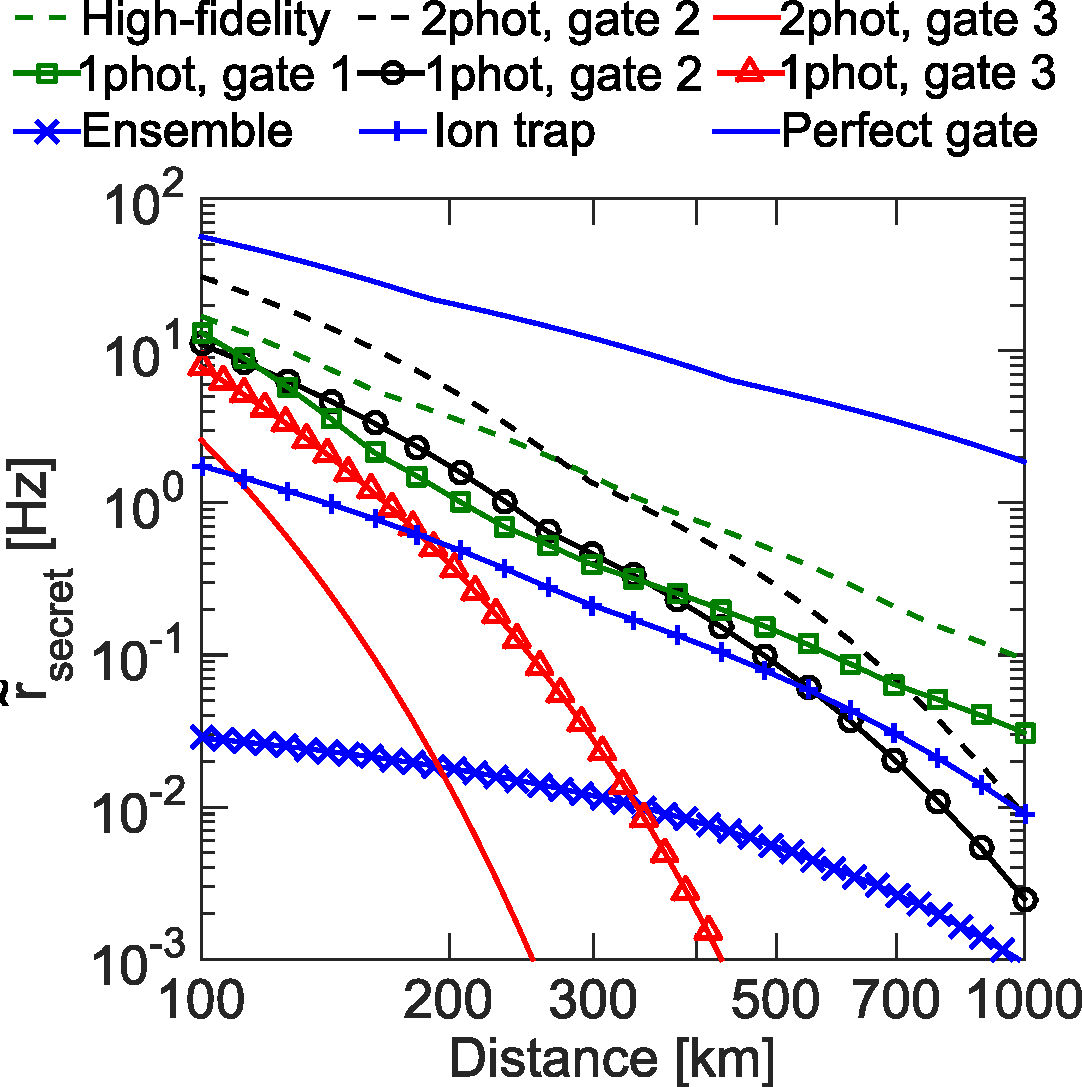
\includegraphics[width=0.48\textwidth]{./figs_Borregaard_PRA2015/figureX7b}
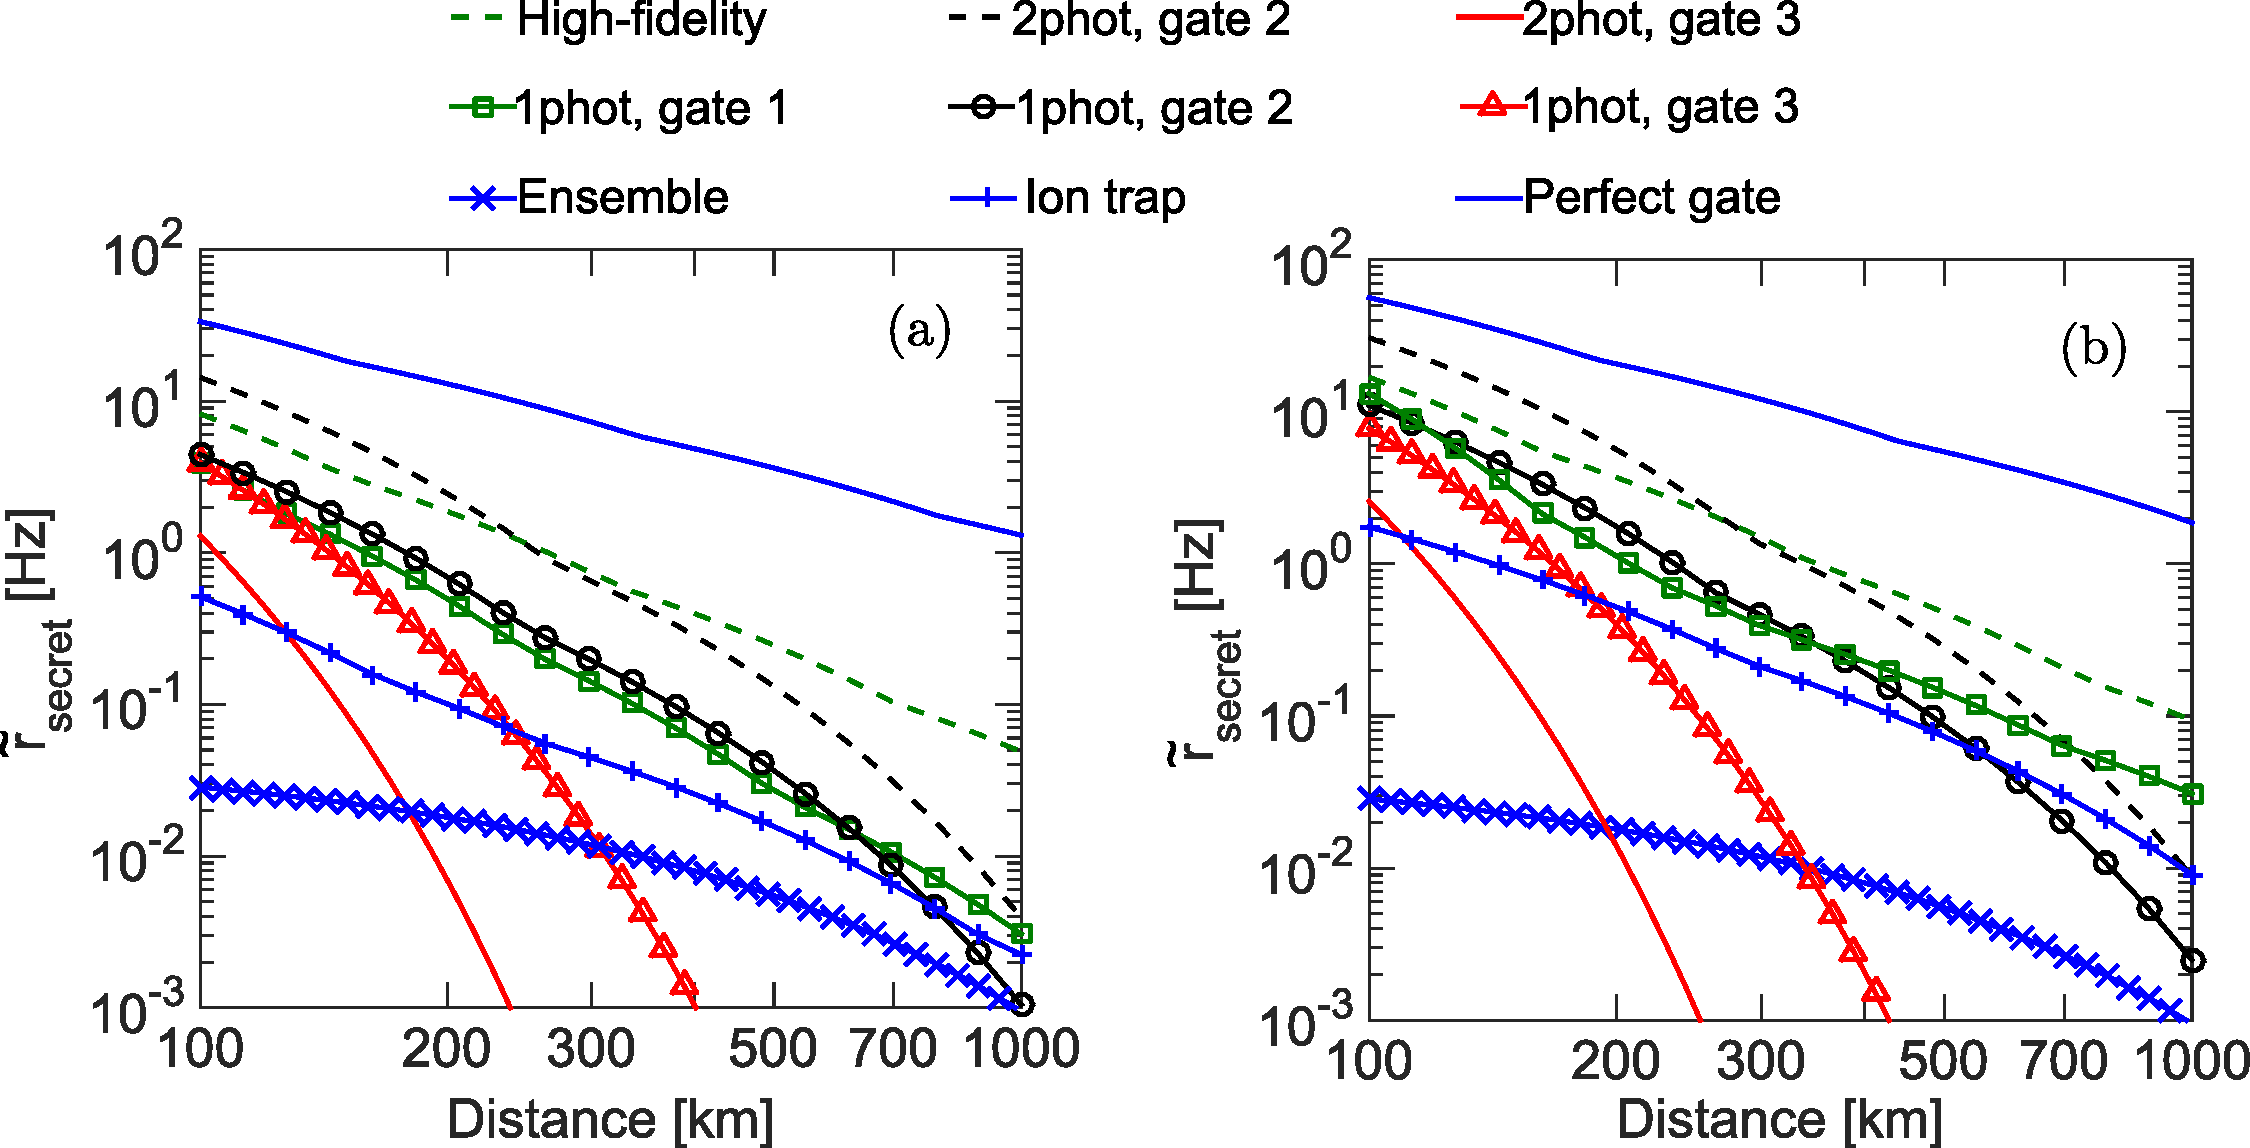
\includegraphics[width=1\textwidth]{./figs_Borregaard_PRA2015/figureX7}
\caption[Optimal secret key rate I]    
{Normalized secret key rate per station
($\tilde{r}_{\mathrm{secret}}$) as a function of the distribution distance
(Distance) for the high-fidelity repeater and other cavity-based repeaters
assuming a cooperativity of $C=$100. (a) is for 2 qubits per repeater station
while (b) is for 4 qubits per repeater station. The other cavity-based repeaters
are labelled as, e.g., ´``1phot, gate 2'', which indicates that it is a
repeater based on the single-photon detection scheme and gate 2. The rate of an
ensemble-based repeater (´``Ensemble'') is also shown~\cite{sangouard1}. For
simplicity, we have assumed a fixed number of four swap levels in the
ensemble-based repeater even though a smaller number of swap levels might
increase the rate for small distances ($\lesssim400$ km). Finally, we have
plotted the rate of an ion trap repeater scheme (´``Ion trap'') with a
collection efficiency of 10\% and gate fidelity of 99.3\% and the ultimate rate
obtainable with perfect deterministic gates and perfect entanglement generation
with the two-photon scheme (´``Perfect gate'') for comparison. For the ion trap
repeater we have plotted the highest rate obtainable with either the one-photon
or two-photon scheme.}
\label{fig:figureX7}
\end{figure} 
\begin{figure} [H]
\centering
% 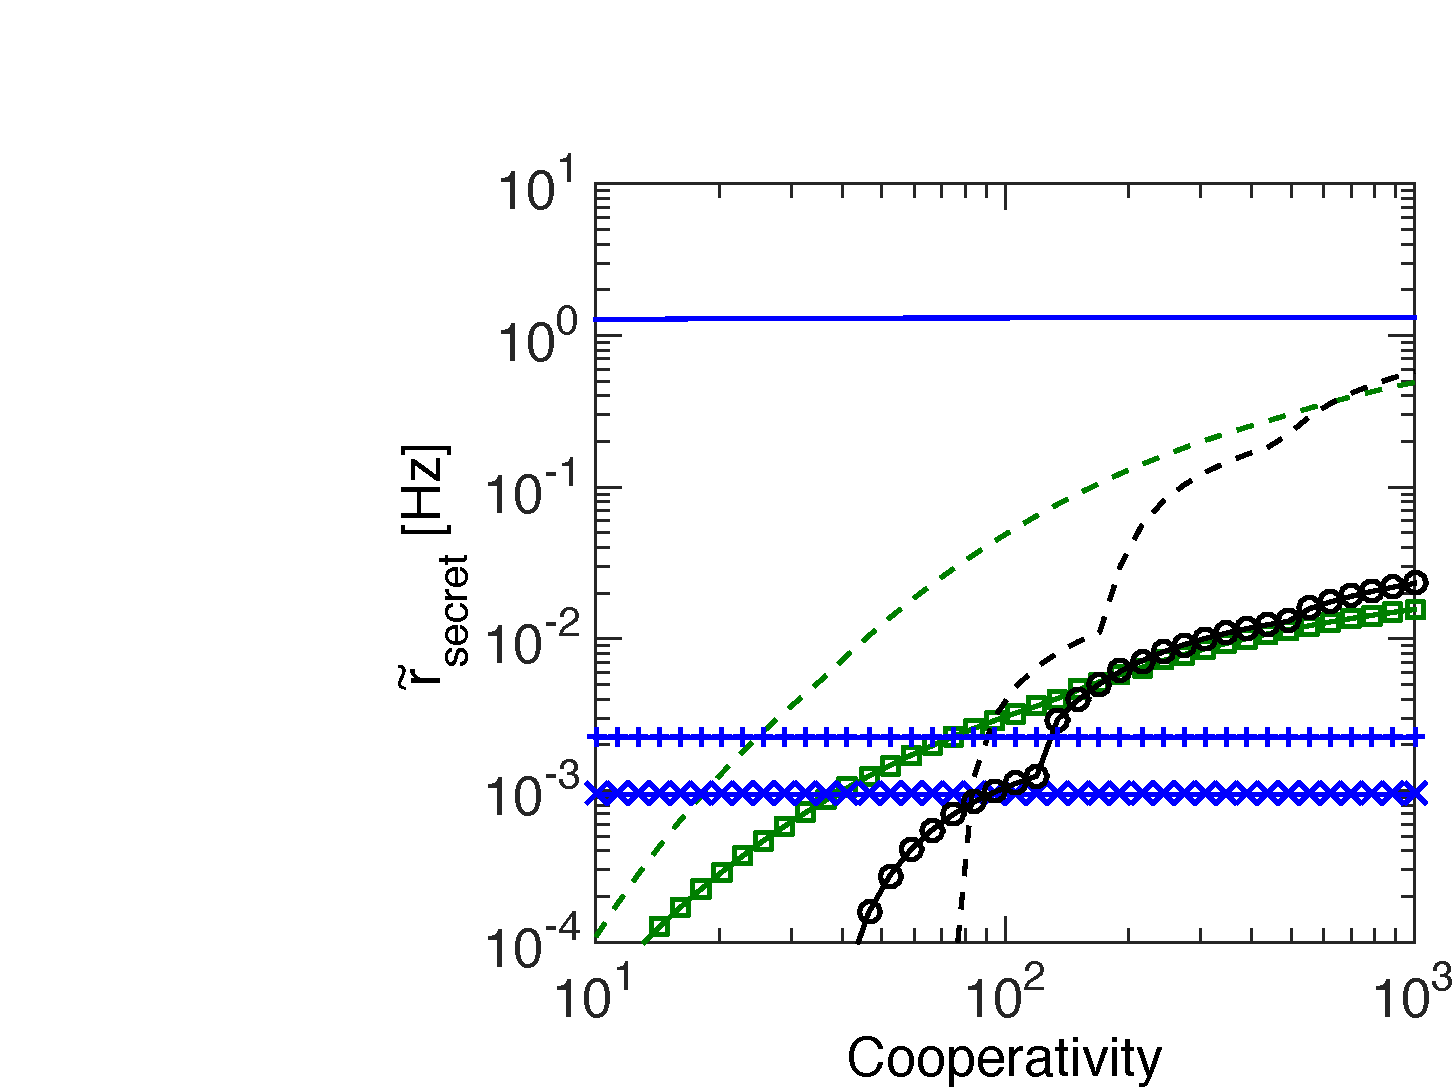
\includegraphics[width=0.48\textwidth]{./figs_Borregaard_PRA2015/figureX8a}
% 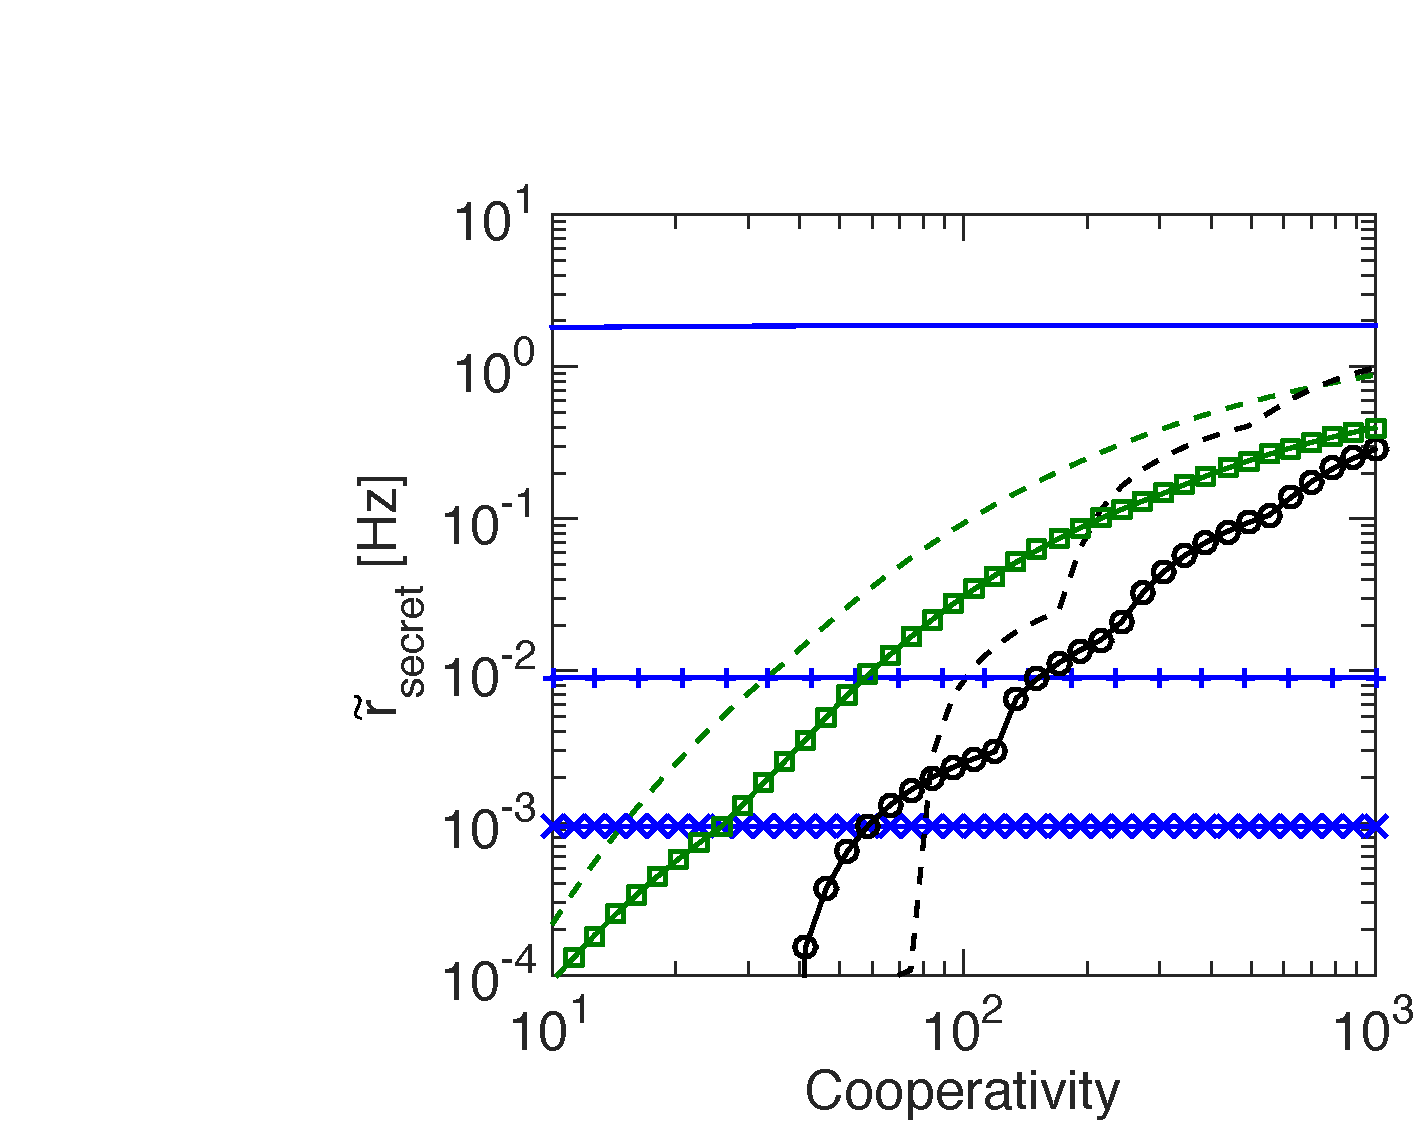
\includegraphics[width=0.48\textwidth]{./figs_Borregaard_PRA2015/figureX8b}
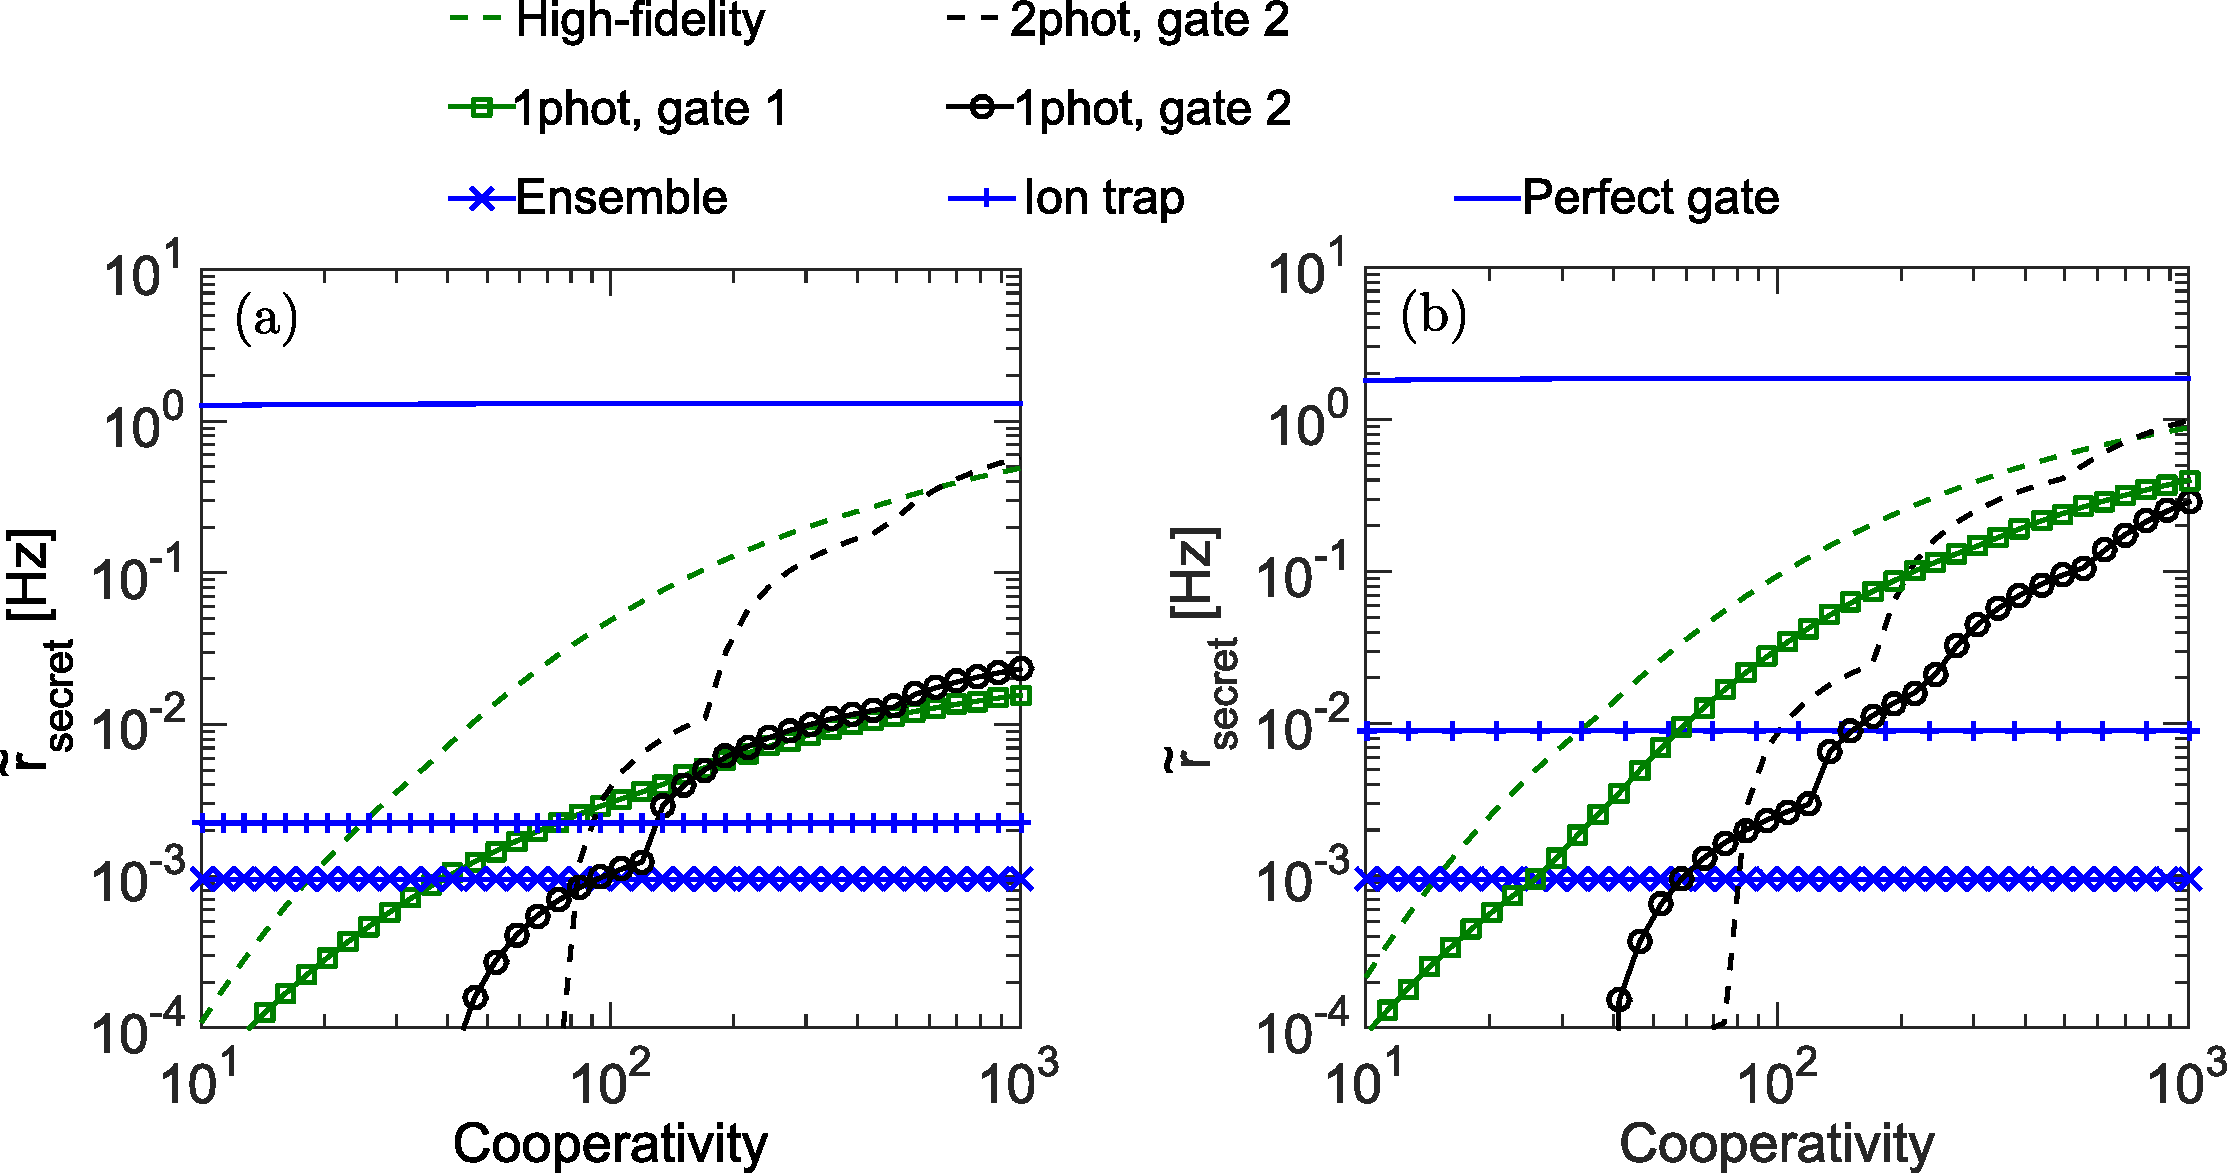
\includegraphics[width=1\textwidth]{./figs_Borregaard_PRA2015/figureX8.pdf} 
\caption[Optimal secret key rate II]{Normalized secret key rate per station
($\tilde{r}_{\mathrm{secret}}$) as a function of the cooperativity ($C$) for the
high-fidelity repeater and other repeaters assuming a distribution distance of
1000 km. (a) is for 2 qubits per repeater station while (b) is for 4 qubits per
repeater station.}
\label{fig:figureX8}
\end{figure}

The secret key rates per repeater station of the high-fidelity repeater and the
other cavity-based repeaters are shown in Fig.~\ref{fig:figureX7} for distances
$[100;1000]$ km and a cooperativity of 100 and in Fig.~\ref{fig:figureX8} for a
distance of 1000 km and cooperativities in the interval $[10;1000]$. As shown in
\reffig{fig:figureX7}, the repeaters based on gate 3 are simply not able to
distribute entanglement over large distances for realistic cooperativities. As a
consequence, repeaters based on gate 3 do not appear on Fig.~\ref{fig:figureX8}
since their secret key rate is simply too low.

In general, the high-fidelity repeater (2-photon, gate 1) achieves the highest
secret key rate for a broad range of cooperativities and long distances $\gtrsim
300$ km. This reflects both that this protocol allows for a higher number of
swap levels and that the secret key rate favors the distribution of
high-fidelity pairs since these gives the highest secret fraction (see
\reffig{fig:figure5}). It is also apparent from Fig.~\ref{fig:figureX8} that
while repeaters based on gate 2 need cooperativities above 100 for a distance of
1000 km, repeaters based on gate 1 are able to function with much lower
cooperativities around $30-40$. This is because the heralded gate has nearly
unit fidelity, independent of the cooperativity. For high cooperativities or
low distances, a repeater based on the two-photon detection scheme and gate 2
can give a slightly higher secret key rate than the high-fidelity repeater. This
improvement is, however, less than a factor of 2 in the secret key rate. The
steps in the rates of the schemes based on gate 2 in Fig.~\ref{fig:figureX8}
originate from the fact that as the cooperativity increases, the fidelity of
gate 2 increases and at some point the fidelity is high enough to allow for
another swap level, which makes the rate increase abruptly.
From the optimizations, we find that the sequential repeater architecture
achieves slightly higher rates (less than a factor 2) than the parallel repeater
architecture for 4 qubits per repeater station, while the opposite is the case
for 2 qubits per repeater station.

In general, repeaters based on the two-photon detection schemes outperform
repeaters based on the single-photon detection scheme except for repeaters based
on gate 3. This reflects that repeaters based on gate 3 cannot perform many swap
levels since the fidelity simply decreases too rapidly with the number of swap
levels. The result of the optimization was that no swap levels were actually
preferred for repeaters based on gate 3 for $C\leq1000$.  As a result, the
elementary links in these repeaters are long and fiber losses therefore
significantly decrease the total detection probability $\eta$ in the
entanglement generation schemes. In the limit of very low $\eta$, the one-photon
scheme is advantageous since the success probability only depends linearly on
$\eta$. For the optimizations, we have assumed that the combined efficiency of
the SPD detectors and outcoupling of light from the cavities is $\eta_{d}=$50\%.
If this efficiency is smaller, repeaters based on single-photon detection may be
desirable. We also find that the purification protocol, in general, performs
better with than without the modification of Ref.~\cite{nickerson}. The
improvement is, however, limited to a factor of $\lesssim2$ for the parameters
considered in Figs.~\ref{fig:figureX7}-\ref{fig:figureX8}.

It is important to stress that the rates plotted in
Figs.~\ref{fig:figureX7}-\ref{fig:figureX8} are the secret key rates divided by
the total number of repeater stations. The actual distribution rate can thus be
obtained by multiplying with the number of repeater stations. For the
high-fidelity repeater, we find a secret key rate of $\sim$16 Hz over 1000 km
for 33 repeater stations and a cooperativity of 1000 assuming 2 qubits per
repeater station.  For a more modest cooperativity of 100, a secret key rate of
$\sim$1.5 Hz over 1000 km can be obtained.

We can compare the rate found here to the rate obtainable with repeaters based
on atomic ensembles. In Ref.~\cite{sangouard1} an efficient repeater based on
atomic ensembles is described, which achieves one of the highest distribution
rates for repeaters based on atomic ensembles~\cite{sangouard3}. The fidelity of
the distributed pair and the distribution rate are derived in
Ref.~\cite{sangouard1} for a repeater with four swap levels corresponding to 17
repeater stations.  Based on this, we have calculated the secret key rate
assuming an optimistic, basic repetition rate of the ensembles of 100 MHz and
memory and SPD efficiencies of 90\%. The rate of the ensemble-based repeater is
also shown in Figs.~\ref{fig:figureX7}-\ref{fig:figureX8} for similar
assumptions about fiber losses etc. as for the cavity-based repeaters. We have
assumed that the repeater uses four swap levels for all distances even though a
smaller number of swap levels may be desirable for smaller distances
($\lesssim400$ km)~\cite{sangouard1}. For a distance of 1000 km, we find a rate
of $\sim0.03$ Hz for 33 repeater stations. This shows that repeaters based on
individual atoms in cavities may be very promising candidates for realizing
efficient quantum repeaters with rates exceeding those obtainable with atomic
ensembles. The main reason for this is that very efficient entanglement swapping
can be realized in the cavity-based repeaters which greatly enhances the
distribution rates for long distances. On the contrary, repeaters based on
atomic ensembles and linear optics have an upper limit on the swapping
efficiency of 50\%.

For comparison we have also considered a repeater based on ion traps where there
is no cavity to collect the light. Non-local entanglement can still be created
by collecting the emitted light with a lens as demonstrated in
Ref.~\cite{monroe2014} where a collection efficiency of 10\% was reported. The
entanglement swapping can be realized using a gate, which has been demonstrated
experimentally with a fidelity of 99.3\% and a gate time of $50$
$\mu$s~\cite{blatt1}. Note that this fidelity was measured for the generation of
a single state in Ref.~\cite{blatt1} but we will assume it to be the fidelity of
the entanglement swap. The rate of such a ion-trap repeater is shown in
Figs.~\ref{fig:figureX7}-\ref{fig:figureX8} with assumptions about fiber losses
etc. summarized in Tab.~\ref{tab:parameter}. We have assumed a collection
efficiency of 10\% and as a result, the one photon scheme with modified
purification performs better than the two-photon scheme for 4 qubits per
repeater station. However for two qubits, where purification is not possible,
the two-photon scheme is in general advantageous except for small distances ($<$
200 km). We have assumed a gate fidelity of 99.3\% and have plotted the highest
rate obtainable with either the one-photon or two-photon scheme.

It is seen that the high-fidelity repeater outperforms the ion-trap repeater for
$C\gtrsim30$, which is mainly due to the low collection efficiency in the
entanglement generation. The ultimate rate, obtainable with a repeater with
perfect deterministic entanglement swapping and entanglement generation based on
the two-photon detection scheme with a collection efficiency set by $4C/(1+4C)$,
is also shown in Figs.~\ref{fig:figureX7}-\ref{fig:figureX8}. A similar repeater was
considered in Ref.~\cite{sangouard2} to demonstrate the feasibility of repeaters
based on trapped ions. For $C=1000$, the high-fidelity repeater achieves only a
factor of $\sim2$ slower rate than this ultimate limit for a distance of 1000
km.

\section{Conclusion}        

In conclusion, we have performed a detailed analysis of quantum repeaters based
on individual emitters in optical cavities. We have found that a high-fidelity
repeater based on the heralded gate described in Ref.~\cite{Borregaard2015a} combined
with a two-photon detection scheme is the best option over a large parameter
regime and enables high secret key rates over large distances even for limited
cooperativities $<100$. Compared with a number of other cavity based repeaters
it achieves rates that are up to two orders of magnitude faster for long
distances (1000 km) and cooperativities $<100$. For small distances or higher
cooperativities, a repeater based on the deterministic CNOT gate described in
Ref.~\cite{Anders2prl} combined with a two-photon detection scheme can achieve
rates which are slightly higher than the high-fidelity repeater but the
improvement is less than a factor of 2.

We have also compared the high-fidelity repeater to the repeater in
Ref.~\cite{sangouard1}, which is based on atomic ensembles. For a distance of
1000 km and $C\gtrsim20$ the high-fidelity repeater begins to outperform the
ensemble-based repeater and an improvement of more than two orders of magnitude
in the secret key rate is possible for $C\gtrsim100$. The main reason for the
advantage of the high-fidelity repeater is that entanglement can be swapped very
efficiently using the heralded CNOT gate described in Ref.~\cite{Borregaard2015a}.
Consequently, the number of swap levels in the repeater can be increased without
the need of intermediate purification, which greatly enhances the rate for large
distances. A similar advantage could in principle be achieved by resorting to a
trapped ion system, where efficient gates can be implemented. For current
systems, the collection efficiencies are, however, so low that a trapped ion
system could be outperformed by a cavity system with a limited finesse of
$C\gtrsim 30$. If the collection efficiency could be overcome, e.g. by placing
the ions in a cavity with a high cooperativity, the rate can be substantially
improved, but with $C>1000$ the high fidelity repeater investigated here is
within a factor of two of this ideal repeater. It should, however, be noted that
we have compared schemes with strong physical differences in our analysis. The
high-fidelity repeater requires an extra auxiliary atom while auxiliary atomic
levels are required to decrease the error of the deterministic cavity-based CNOT
gates. The ensemble-based and ion-trap repeaters are also very different
physical systems compared to the cavity-based repeaters with individual atoms.
The different experimental difficulties in realizing the physical requirements
for the various repeater schemes should be included in a more advanced
assessment.

Finally, we note that while we have investigated a number of different possible
repeater protocols there may be even more advantageous procedures. Hence the
results that we have derived here should be seen as lower limits to the
achievable communication rates. A particular interesting  possibility could be
to investigate proposals along the lines of Ref.~\cite{cirac1,cirac2}, which
also rely on heralding measurements to detect errors during entanglement
generation and two qubit operations.  Possibly some of the ideas from these
schemes could be used to improve the communication beyond what we have found
here.
